\documentclass[useAMS,usenatbib,a4paper]{mn2e}
\usepackage{graphicx}
\usepackage{aas_macros}
\usepackage{multirow}
\usepackage{hyperref}
 
\title[Mid-infrared spectroscopy of M31]{Mid-infrared spectroscopy of the Andromeda galaxy}
\author[D. Hemachandra et al.]
{D. Hemachandra$^{1}$\thanks{E-mail: dhemacha@uwo.ca},
P. Barmby$^{1}$, 
E. Peeters$^{1,2}$, 
S.P. Willner$^{3}$, 
M.L.N. Ashby$^{3}$,
H.A. Smith$^{3}$, 
\newauthor 
K.D. Gordon$^{4}$,
D.A. Smith$^{4}$,
and
G.G. Fazio$^{3}$\\
$^{1}$Department of Physics and Astronomy, University of Western Ontario, London, ON, N6A 3K7, Canada\\
$^{2}$SETI Institute, 189 Bernardo Avenue, Suite 100, Mountain View, CA 94043, USA\\
$^{3}$Harvard-Smithsonian Center for Astrophysics, Cambridge, MA 02138, USA\\
$^{4}$Space Telescope Science Institute, 3700 San Martin Drive, Baltimore, MD 21218, USA
}


\begin{document}

\date{}

\maketitle

\label{firstpage}

\begin{abstract}
We present {\sl Spitzer}/Infrared Spectrograph 5--21~$\mu$m spectroscopic maps towards 12 regions in the Andromeda galaxy (M31). 
These regions include the nucleus, bulge, an active region in the star-forming ring, and 9 other regions chosen to cover a range of mid-to-far-infrared colours. 
Our observations did not reproduce the suppressed 6--8~$\mu$m features and enhanced 11.3~$\mu$m feature intensity and FWHM seen with the ISOCAM instrument on the Infrared Space Observatory.
In line with previous results, PAH feature ratios (6.2~$\mu$m and 7.7~$\mu$m features compared to the 11.2~$\mu$m feature) measured from our extracted M31 spectra, except the nucleus, strongly correlate. The equivalent widths of the main PAH 
features decrease with increasing radiation hardness, consistent with that observed for other nearby spiral and starburst galaxies. 
The nucleus does not show any PAH emission but does show strong silicate emission at 9.7~$\mu$m. Furthermore, different spectral features (11.3~$\mu$m PAH emission, silicate emission and [NeIII] 15.5~$\mu$m line emission) have distinct spatial distributions in the nuclear region: the silicate emission is confined towards the nuclear centre (19--27pc) while the PAH emission peaks 15\arcsec north of the centre. At this position, the PAH emission is atypical with strong emission at 11.2~$\mu$m and at 15-20~$\mu$m but suppressed emission at 6--8~$\mu$m. We also find that the silicate emission profile is redshifted and broader compared to that observed towards the Galactic centre. 
Both the silicate emission and atypical PAH emission provide evidence for a low luminosity active galactic nucleus in M31.
\end{abstract}

\begin{keywords}
galaxies: individual: M31 --
galaxies: ISM --
galaxies: nuclei --
infrared: ISM --
ISM:  molecules -- 
ISM: lines and bands
\end{keywords}



\section{Introduction}

Mid-infrared spectra provide a unique diagnostic tool to understand the physical conditions in the interstellar medium of galaxies. 
The rich range of spectral features (Polycyclic Aromatic Hydrocarbons (PAHs), atomic fine structure lines (e.g. Ne, S) and the
amorphous silicate feature centred at 9.7~$\mu$m) provide information on dust properties, radiation field and star formation. 
With the advent of infrared space telescopes, such as the Infrared Space Observatory (ISO, \citealt{Kessler1996}) and 
the {\em Spitzer} Space Telescope \citep{spitzer2004},  mid-infrared spectroscopy has become an important method
of investigating the infrared emission from galaxies. 

PAHs are known as the main carrier of the ubiquitous mid-infrared emission bands (e.g. \citealt{Allamandola1989}, \citealt{puget89}).
They are large hydrocarbon molecules consisting of $\sim$50--100 carbon atoms \citep{Tielens2008}. 
The main PAH features are seen at 3.3, 6.2, 7.7, 8.6, 11.3 and 12.7~$\mu $m (e.g., \citealt{Gillett:73}, \citealt{Geballe:85}, \citealt{Peeters:toledo:11}). 
These bands are attributed to the vibrational de-excitation of PAH molecules through bending and stretching modes of C-H and C-C bonds (e.g. \citealt{Allamandola1989}, \citealt{puget89}). 
The 6 to 8 micron features are thought to originate mostly from ionized PAHs and the 3.3 and 11.3~$\mu$m 
emission bands from neutral PAHs (e.g. \citealt{Hudgins:rev:04} and reference therein, \citealt{Hony:oops:01},  \citealt{Galliano:08}). 

The relative strength of the PAH features vary spatially within extended objects and from galaxy-to-galaxy \citep[e.g.][]{Galliano:08}. While extinction does influence the individual PAH bands to different degrees \citep[e.g.][]{Brandl2006, Stock:13}, the observed spread in PAH intensity ratios is dominated by the PAH charge balance \citep{Galliano:08}. In addition, feature ratios do change more drastically close to active galactic nuclei where the overall strength of PAH emission also gets weaker (\citealt{Roche1991}, \citealt{Smith:2007lr}). \citet{Smith:2007lr} found that the mid-infrared 
spectra from some weak AGNs show suppressed 6 to 8~$\mu$m PAH features (by up to a factor of 10 in strength) but are bright at 11.3~$\mu$m. One possible explanation for this behaviour is that AGNs alter the grain composition by selective destruction of small PAHs and/or even can excite the PAHs. Alternatively, the PAH emission is modified by the low star formation intensity in the centers of many AGNs \citep{Smith:2007lr}. 

Previous studies of nearby galaxies indicate that metallicity and radiation hardness can both affect the PAH emission (e.g. \citealt{Madden:00}, \citealt{Beirao:06}, \citealt{Engelbracht_2008}, \citealt{Munoz:09}). In particular, the PAH equivalent widths (EQWs) in nearby galaxies decrease with increasing radiation hardness, although \citet{Brandl2006} found no such correlation within their starburst sample. In addition, PAH EQWs show an anti-correlation with metallicity in star-forming galaxies. This variation of PAHs among galaxies has also been observed within H~{\sc ii} regions 
of M101 \citep{Gordon:2008lr}. But there are no other investigations done on a single star-forming galaxy with sufficiently high resolution to see whether the correlations mentioned above hold within a galaxy similar to the Milky Way.

The amorphous silicate feature at 9.7~$\mu$m is another aspect of the mid-infrared spectra of galaxies and in particular their nuclei.  \citet{Spoon2007} 
classified infrared galaxies based on the equivalent width of the 6.2~$\mu$m PAH feature and the strength of the 9.7~$\mu$m silicate feature. 
They  found galaxies spread along two distinct branches: one in which silicate absorption strength was anti-correlated with PAH
equivalent width, and another in which the weak silicate feature strength did not depend on the 6.2~$\mu$m equivalent width.
Silicate {\em emission} at 9.7~$\mu$m has also been observed  towards several galaxies including LINERS, Seyfert galaxies, ULIRGs, and QSOs \citep[e.g.][]{Sturm2005, Hao2005, Spoon2007, Mason2012} 
and can be used to constrain the geometry and structure of the emitting nuclear region \citep{Mason2009}.



M31 with its proximity \citep[$785\pm25$ kpc; ][]{Mcc2005} and rich observational databases provides the most detailed view of a star forming galaxy similar 
to the Milky Way. The active star forming ring visible in 8~$\mu$m  {\em Spitzer}/IRAC images \citep{Barmby2006lr} provides evidence of abundant PAHs in M31. 
However, ISOCAM spectro-imaging observations of M31\citep{1998Cesarsky} showed that four regions including the nucleus and bulge 
of this galaxy have very odd PAH spectra, bright at 11.3~$\mu$m while showing weak or no  6.2, 7.7, and 8.6~$\mu$m bands. 
Investigating this unusual PAH emission was the main motivation for the work described in this paper. 
The centre of M31 has a complicated physical structure. It hosts a very inactive supermassive black hole with a mass of 
$0.7-1.4 \times 10^8$~M$_{\sun}$ \citep{Bacon2001, Bender2005} and also has a lopsided nuclear disk  with two stellar 
components \citep{Lauer1993} and an A-star cluster \citep{Bender2005}. While M31's nucleus is known to be inactive from an 
X--ray perspective \citep{Li2011}, mid-infrared indicators of its nuclear activity, such
as infrared excess or spectral features of silicates,  have received relatively little attention. 
The higher spatial resolution available in observations of  a very nearby galaxy like M31, compared to 
luminous, distant objects such as ultra-luminous infrared galaxies \citep{Spoon2007} or nearby Seyferts \citep{Mason2009},
makes exploring its mid-infrared spectrum worthwhile.


We employed mid-infrared spectral maps from the {\em Spitzer}/Infrared Spectrograph (IRS) from 12 regions of M31 for a further investigation of 
its infrared properties. This sample includes the nucleus, bulge, an active region in the star-forming ring (all previously observed by ISOCAM), and 9 
other regions chosen to cover a range of properties as described in Section~\ref{sect:irs_obs}. 
We obtained the processed version of ISOCAM observations of M31 and compare them with the IRS results in Section~\ref{sect:iso_vs_irs}. 
Section~\ref{sect:pah_ratios} discusses PAH intensity ratios.
In Section~\ref{sect:eqw_rh}, we investigate the relationship between PAH equivalent widths and radiation 
hardness and compare to that found by \citet{Engelbracht_2008} and \citet{Gordon:2008lr}. Metallicity and PAH EQWs are compared in 
Section~\ref{sect:eqw_met}, and Section~\ref{sect:nucleus} discusses the dust properties of the nucleus. The paper is summarized in Section~\ref{sect:summary}.


\section{Observations and data reduction}

\subsection{IRS observations}
\label{sect:irs_obs}

\begin{figure}
\centering
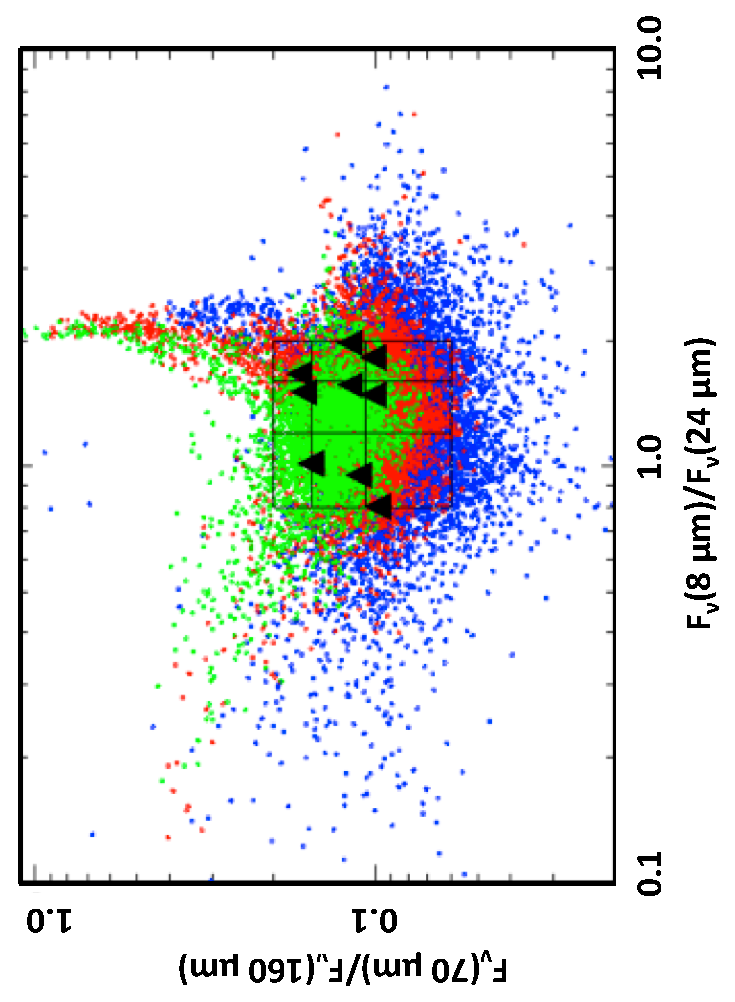
\includegraphics[width = 6.5 cm,angle=270]{fig1.eps}
\caption{$8 - 24/70 - 160$ $\mu$m colour-colour diagram of M31 obtained from IRAC and MIPS imaging. Colour-coding of points represents
24~$\mu$m flux, from faintest (blue) to brightest (red). The plot is divided into 9 regions (black grid), and the observations were made to 
cover those regions subject to a 24~$\mu$m brightness cut. The black triangles indicate colours of the regions we observed.}
\label{colourmaps}
\end{figure}

We obtained mid-infrared spectral maps of 12 regions in M31 using the {\em Spitzer}/IRS instrument \citep{IRS2004} covering wavelengths from 5 to 21 microns. 
These regions include the nucleus, the `bulge' and `active' regions previously observed by ISOCAM (the latter is Region 9 in our sample), 
and 9 other regions selected to cover a range of metallicities and dust temperatures. These 9 regions were chosen by convolving the IRAC 8~$\mu$m \citep{Barmby2006lr}
and MIPS \citep{gordon06a} maps to the same resolution and constructing an $8 - 24/70 - 160$ $\mu$m colour-colour diagram (Figure~\ref{colourmaps}).
This colour space was used to give a rough definition of the types of spectral energy distribution; the 
dense region in the plot was split into a 3x3 grid and one pixel in each grid region (subject to a 24$\mu$m brightness cut)
was selected for spectroscopy. The locations of the observed regions are shown in Figure~\ref{m31}, and 
their coordinates are given in Table~\ref{regions}. A background observation was also made off the galaxy 
along the minor axis for use in background subtraction from the data cubes.



\begin{table*}
 \centering
 \begin{minipage}{90mm}
\caption{Spitzer/IRS Target Locations in M31
\label{regions}}
\begin{tabular}{lccrl}
\hline Name & R.A. (J2000) & Decl. (J2000) & ${R_{\rm gc}}^b$ & $12+\log({\rm O/H})^c$
\\
 \hline
Nucleus$^a$ & $00^{\rmn{h}}42^{\rmn{m}}44\fs31$ & $41\degr16\arcmin09\farcs4$  & 0.0 & \\
Bulge$^a$   & $00^{\rmn{h}}42^{\rmn{m}}35\fs00$ & $41\degr21\arcmin01\farcs0$  & 4.7 &$8.90\pm0.03$\\
Region 1    & $00^{\rmn{h}}41^{\rmn{m}}30\fs41$ & $40\degr43\arcmin07\farcs8$  & 12.4 &$9.20\pm0.20$\\
Region 2    & $00^{\rmn{h}}45^{\rmn{m}}22\fs85$ & $41\degr38\arcmin53\farcs1$  & 13.0 &$9.07\pm0.02$\\
Region 3    & $00^{\rmn{h}}40^{\rmn{m}}37\fs37$ & $41\degr01\arcmin29\farcs4$  & 12.1 &$8.85\pm0.01$\\
Region 4    & $00^{\rmn{h}}41^{\rmn{m}}17\fs86$ & $41\degr07\arcmin09\farcs8$  & 8.7 &$8.89\pm0.06$\\
Region 5    & $00^{\rmn{h}}43^{\rmn{m}}39\fs57$ & $41\degr19\arcmin03\farcs1$  & 7.0 &$8.93\pm0.08$\\
Region 6    & $00^{\rmn{h}}43^{\rmn{m}}35\fs72$ & $41\degr23\arcmin15\farcs0$  & 4.3 &$8.73\pm0.08$\\
Region 7    & $00^{\rmn{h}}40^{\rmn{m}}53\fs98$ & $40\degr58\arcmin58\farcs9$  & 8.7 &$8.40\pm0.08$\\
Region 8    & $00^{\rmn{h}}42^{\rmn{m}}21\fs60$ & $41\degr07\arcmin17\farcs4$  & 3.1 &$8.94\pm0.08$\\
Region 9$^a$& $00^{\rmn{h}}41^{\rmn{m}}00\fs00$ & $40\degr36\arcmin20\farcs3$  & 13.5 &$8.86\pm0.02$\\
NGC~206     & $00^{\rmn{h}}40^{\rmn{m}}20\fs20$ & $40\degr44\arcmin54\farcs0$  & 9.8 & \\
Background  & $00^{\rmn{h}}44^{\rmn{m}}41\fs80 $ & $40\degr58\arcmin56\farcs0$  & 29.5 & \\
\hline
\end{tabular}
{$^a$Regions with ISOCAM data.\\
$^b$De-projected galactocentric distance in kpc.\\ 
$^c$Metallicities from \citet{Sanders_2011}, except for Regions 5 and 8 where metallicities are estimated from the radial metallicity profile.
}
\end{minipage}
\end{table*}

\begin{figure*}
\centering
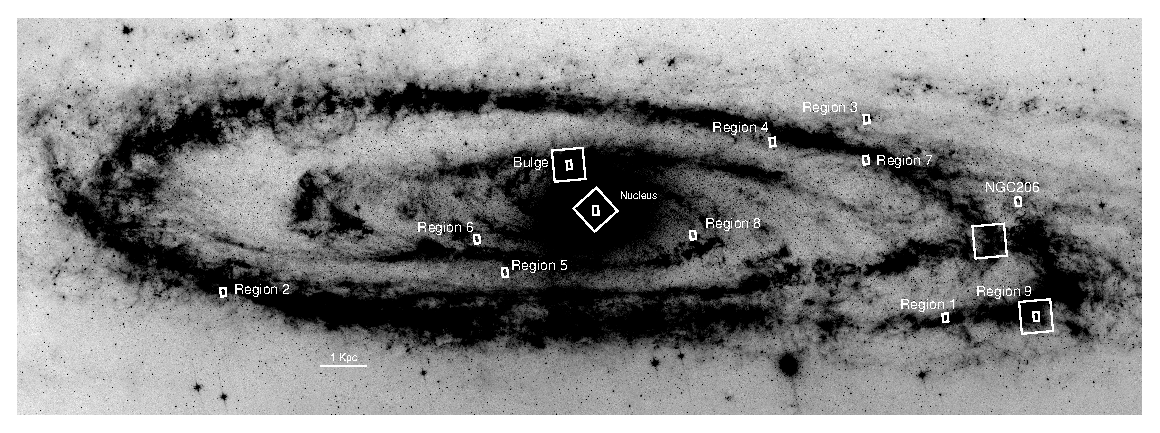
\includegraphics[scale=0.9]{./fig2.eps}
\caption{An 8 micron negative IRAC image of M31 \citep{Barmby2006lr}. Small white rectangles ($30\arcsec\times50\arcsec$) show the regions that we observed, and larger squares ($192\arcsec\times192\arcsec$) show the regions observed by  \citet{1998Cesarsky}.
\label{m31}
}
\end{figure*}


For our observations we used the IRS Short-Low (SL) and Long-Low (LL) modules, which cover wavelengths from 5 to 21 microns. 
The Low modules have resolving power in the range 60--130. Each low-resolution module is divided into two sub-slits 
which provide spectroscopy in either first or second order. They are denoted as SL1 (7.5--14.5~$\mu$m), SL2 (5.2--7.6~$\mu$m),
LL1 (20.5--38.5~$\mu$m, not used in these observations), and LL2 (14.5--20.75~$\mu$m).
All M31 regions were observed in September 2007 as part of G. G. Fazio's Guaranteed Time (program ID 40032). 
The map size was based on the size 
of the IRS slits (SL: $3.6\arcsec \times 57\arcsec$, LL: $10.5\arcsec \times 168\arcsec$). Each region was covered by 18 overlapping observations 
of the SL slit and 11 overlapping observations of the LL slit making the map size $32\arcsec \times 57\arcsec$ for SL and $58\arcsec \times 168\arcsec$ for LL. 
Figure~\ref{slits} shows an example of the slit arrangement. For the brighter regions (nucleus, bulge), ramp times of 14 s (SL) and 30 s (LL) were used, 
while for the fainter regions, ramp times of 60 and 120 s were used respectively. Background observations were taken with each module (2 per ramp time). 
Because all of the targets are in the same part of the sky, a common background observation was used for multiple targets to subtract the background emission. 

\begin{figure}
\centering
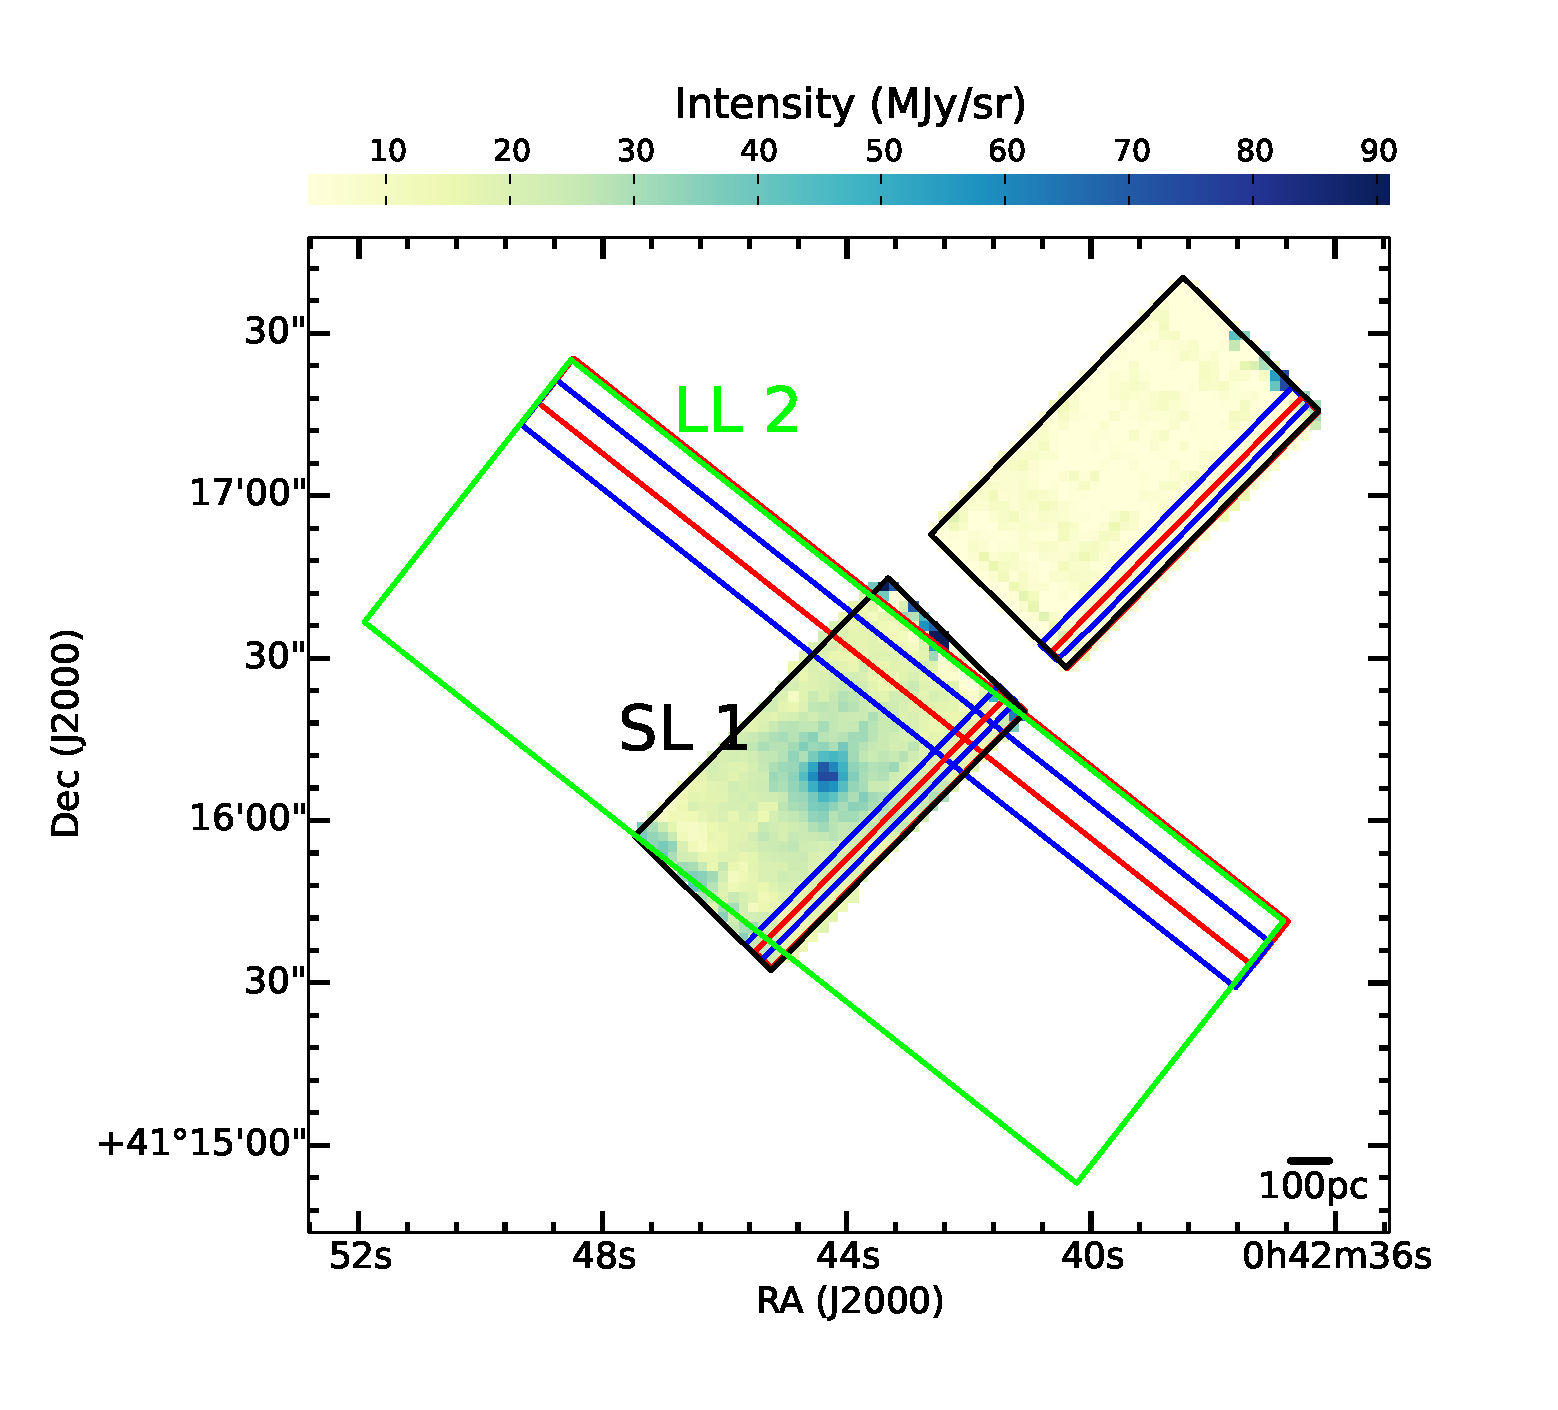
\includegraphics[scale=0.3]{./fig3.eps}
\caption{The 7.6~$\mu$m plane constructed from the SL1 data cube of the nucleus, showing the arrangement of slits used to cover the region. 
Black boxes outline the footprint of the SL1 maps (the off-center SL1 map is from observations made
when SL2 was centred) and the green box outlines the LL2 map. 
Blue and red slits show how  each map was covered using overlapping slit positions.
\label{slits}
}
\end{figure}

\subsection{IRS Data Reduction}
\label{sect:irs_data}

The data were reduced through the SSC pipeline (ver. S17.2.0), and the maps were assembled using the CUBISM program \citep{Smith:2007fk}. 
Bad pixel removal was also done using CUBISM, and the background observations were used to subtract the background emission from these cubes 
following the method outlined by \citet{Gordon:2008lr}. Spectra were extracted using a $30\arcsec\times50\arcsec$   rectangular aperture,
which corresponds to $114\times190$~pc at the distance of M31.
The aperture size was selected to cover the overlapping area of the SL and LL modes; all the IRS maps cover more area than  considered here.
In order to study the spatial variation of the emission near the nucleus, we also extracted spectra from two smaller regions
within that map; these will be further discussed in Section~\ref{sect:nucleus}.
The spectrum of NGC 206 is very noisy and was removed from our analysis. 


There is wavelength overlap between the SL1 and SL2 spectra and also between the SL1 and LL2 spectra.
To generate a single spectrum for each M31 region it is necessary to combine the spectra and
account for photometric offsets between them. We first combined the extracted SL1 and SL2 
spectra by computing the average flux densities over the wavelength overlap region ($7.5 < \lambda< 7.6\mu$m),
adding a constant  to the SL2 spectra so that they matched the SL1 average,
and averaging the SL1 $+$ shifted SL2 spectra over the overlap region.
After this procedure there was still a noticeable mis-match between the SL and LL spectra. We addressed this
by scaling the SL spectra to match IRAC 8~$\mu$m fluxes as follows. IRAC fluxes were measured
on the 8~$\mu$m image \citep{Barmby2006lr} in the same apertures used to extract the IRS spectra.
The extended source  aperture correction of 0.824 was applied to the IRAC fluxes.
The standard deviation of the IRAC flux in a region similar in size but off the disk of the galaxy 
($00^{\rmn{h}}48^{\rmn{m}}58\fs0, +42\degr14\arcmin54\farcs0$) was used to estimate the
IRAC photometric uncertainties.
The {\em Spitzer} synthetic photometry software \citep{SpitzerDAC} 
was then used to quantify the colour correction for each spectrum, i.e. the
multiplicative factor $K$ between the IRAC photometry over its broad bandpass and the IRS flux
density at the centre of the bandpass. The IRAC photometry, IRS flux density, and colour corrections 
for each region are given in Table~\ref{colourK}. Plotting the IRS  and colour-corrected IRAC measurements
(Figure~\ref{offset}) and fitting a straight line weighted by the uncertainties, we found that the best-fit relation 
between the measurements had a slope of $0.81\pm0.08$  and intercept of $-0.05\pm0.06$. 
The non-zero intercept of this fit suggested that an additive offset was more appropriate for combining SL and LL
spectra than a multiplicative one; this method was also used by \citet{Sandstrom12}.
Therefore we scaled each SL spectrum by an offset 
\begin{equation}
x = F_{\rm IRAC8}/K -   F_{\rm IRS8}
\label{eq:offset}
\end{equation}
where the individual offsets are given in Table~\ref{colourK}.
The scaled SL spectra were much better matched to the LL spectra, and the final combination
of SL and LL was done using the average-and-offset procedure described above for SL1 and SL2.

\begin{figure}
\centering
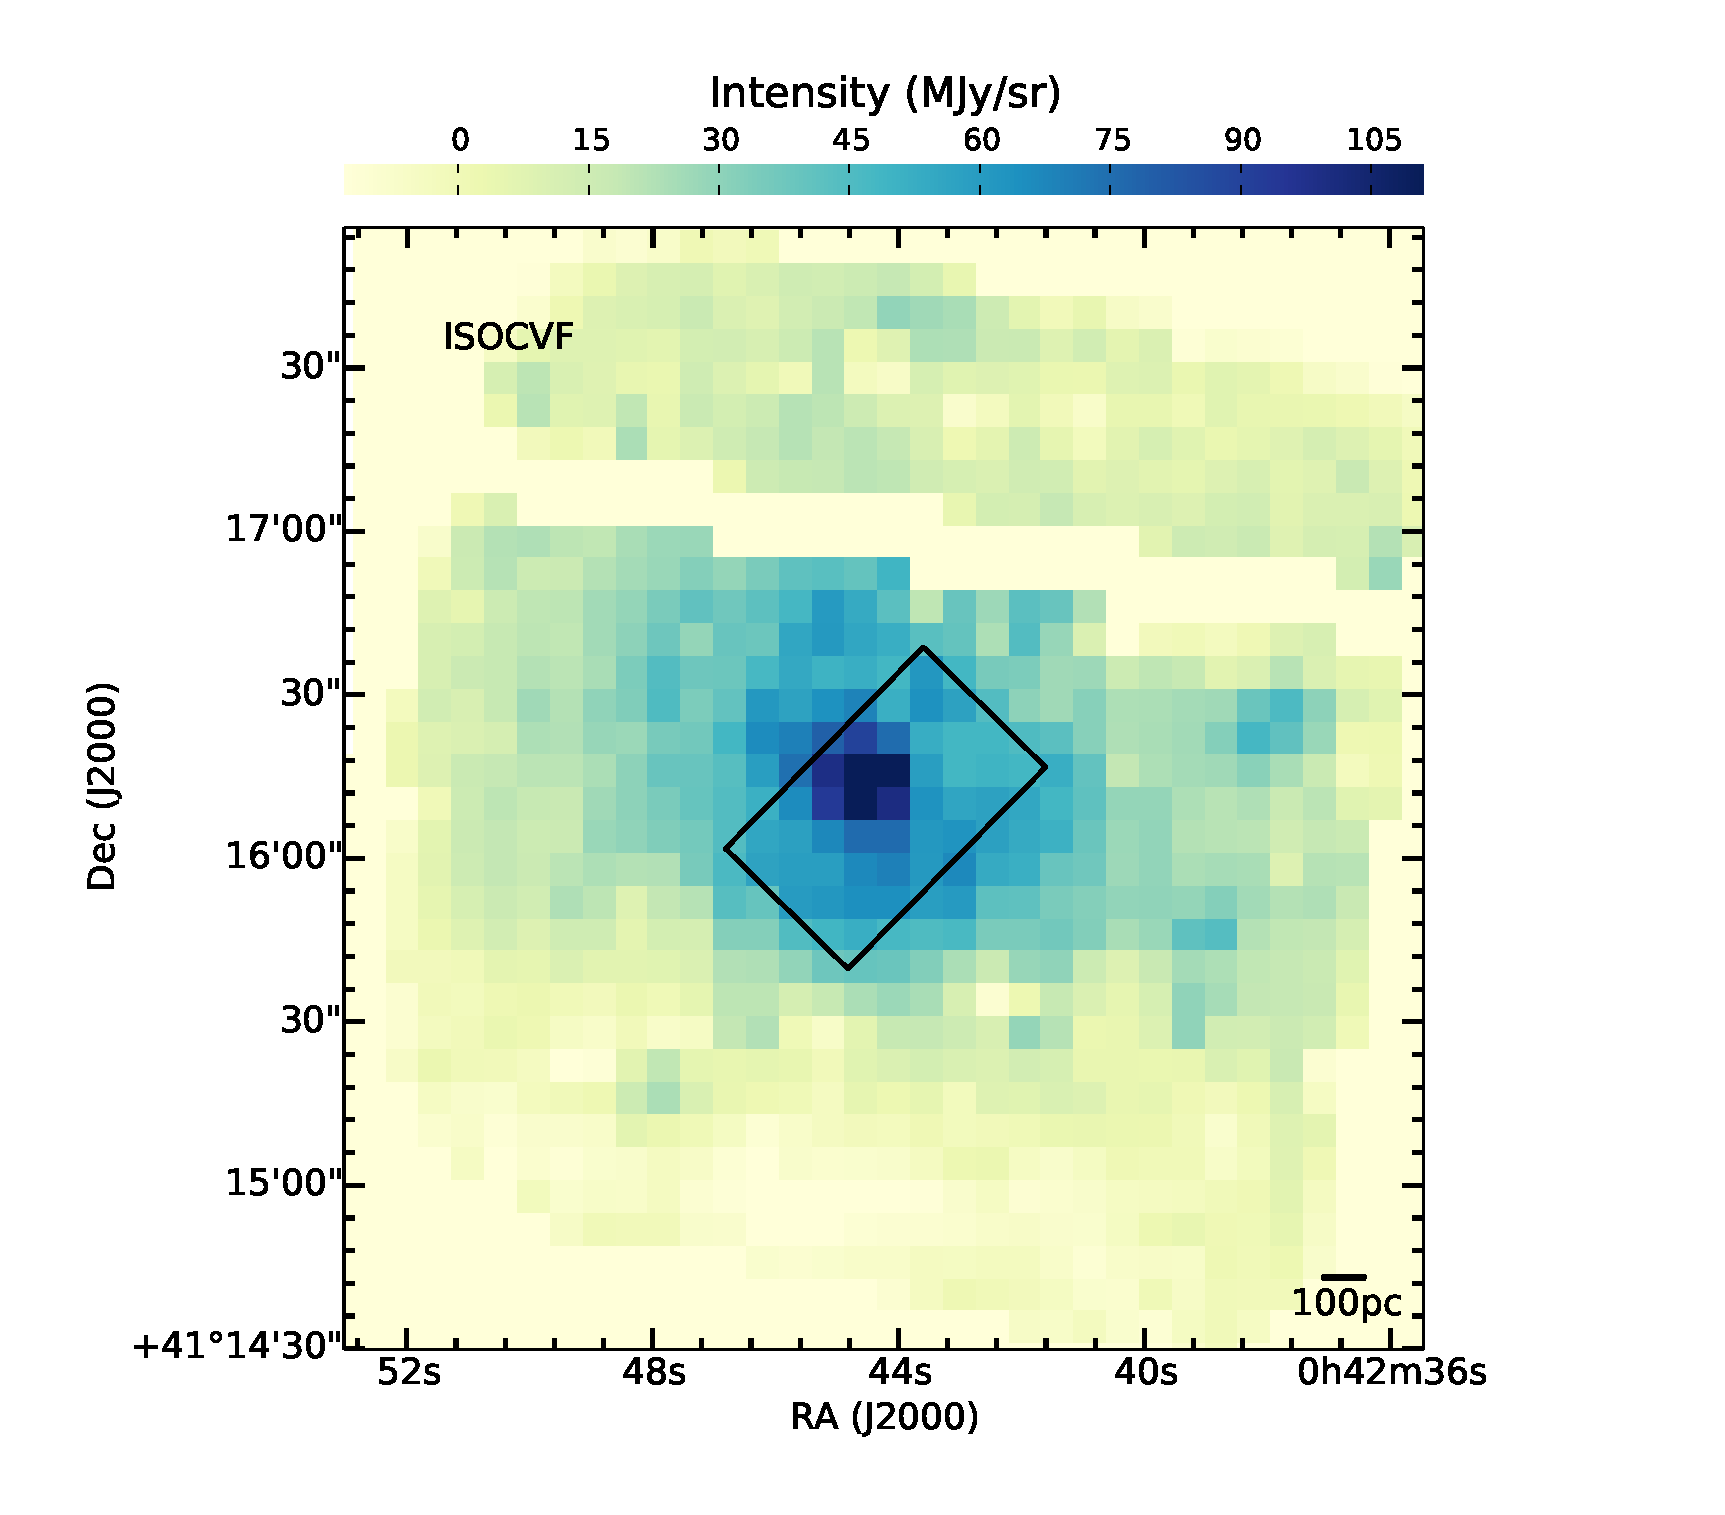
\includegraphics[scale=0.25]{./fig4.eps}
\caption{Intensity of the aperture corrected IRAC 8~$\mu$m image versus that of the colour-corrected IRS spectra at 8~$\mu$m  
obtained using the same aperture for our regions in M31. The straight line is the line of best fit. }
\label{offset}
\end{figure}


\begin{table}
 \centering
 \begin{minipage}{100mm}
\caption{Matched aperture photometry}
  \begin{tabular}{lcccc}
  \hline{Name}&{IRS$^{a}$}&{IRAC$^{b}$}&{$K^{\rm c}$}&{Offset $x^d$} \\ 
{} & { MJy~sr$^{-1}$} & { MJy~sr$^{-1}$} & &  MJy~sr$^{-1}$
   \\
 \hline
 Region 1 & 1.8505 & 1.3923 & 0.532 & 0.3061
 \\ Region 2  & 1.8238 & 1.3731 & 0.555 & 0.2148
 \\ Region 3 & 0.7192 & 0.9689 & 0.767 & 0.3218
 \\ Region 4 & 1.1431 & 0.8513 & 0.589 & 0.0407
 \\  Region 5 & 0.6787 & 0.8088 & 0.773 & 0.1834
 \\  Region 6  & 0.6399 & 0.7656 & 0.927 & 0.0479
 \\  Region 7  & 1.1538 & 0.8243 & 0.526 & 0.1380
 \\ Region 8 & 0.5556 & 0.7135 & 0.877 & 0.1148
 \\  Region 9 & 1.9413 & 1.6562 & 0.606 & 0.3107 
 \\ Bulge & 2.6956 & 2.5473 & 0.532 & 1.2425\\
\hline
 \label{colourK}
\end{tabular}\\
 {$^{\rm a}$Specific intensity measured at 8.00~$\mu$m, no colour correction.\\
 $^{\rm b}$Specific intensity measured over the IRAC 8~$\mu$m bandpass,\\ no extended source correction.\\
$^{\rm c}$Colour correction factor computed from IRS spectrum.\\
 $^{\rm d}$Computed offset between IRAC and IRS as defined in~Eq.~\ref{eq:offset}. }
\end{minipage}
\end{table}

	


\subsection{ISOCAM Data Reduction}
\label{sect:iso_data}

To compare our results with those of  \citet{1998Cesarsky}, we retrieved the highly processed ISOCAM data provided by \citet{Boulanger_F_2005}  
for the nucleus, bulge, and region 9. 
The ISOCAM data were obtained with the circular variable filters (CVFs) over a $3\arcmin \times 3\arcmin$ field of view at a scale of 6\arcsec\ per pixel. 
The wavelength range covered was 5.15--16.5~$\mu$m at a resolution of $\lambda/\Delta \lambda \approx 45$; the ISOCAM instrument is described by \citet{cesarsky1996}.
An example image of the ISOCAM data is shown in Figure~\ref{isonuc}.  For the three regions, we extracted spectra using the same 
$30\arcsec\times50\arcsec$ aperture as for the IRS data. 

\begin{figure}
\centering
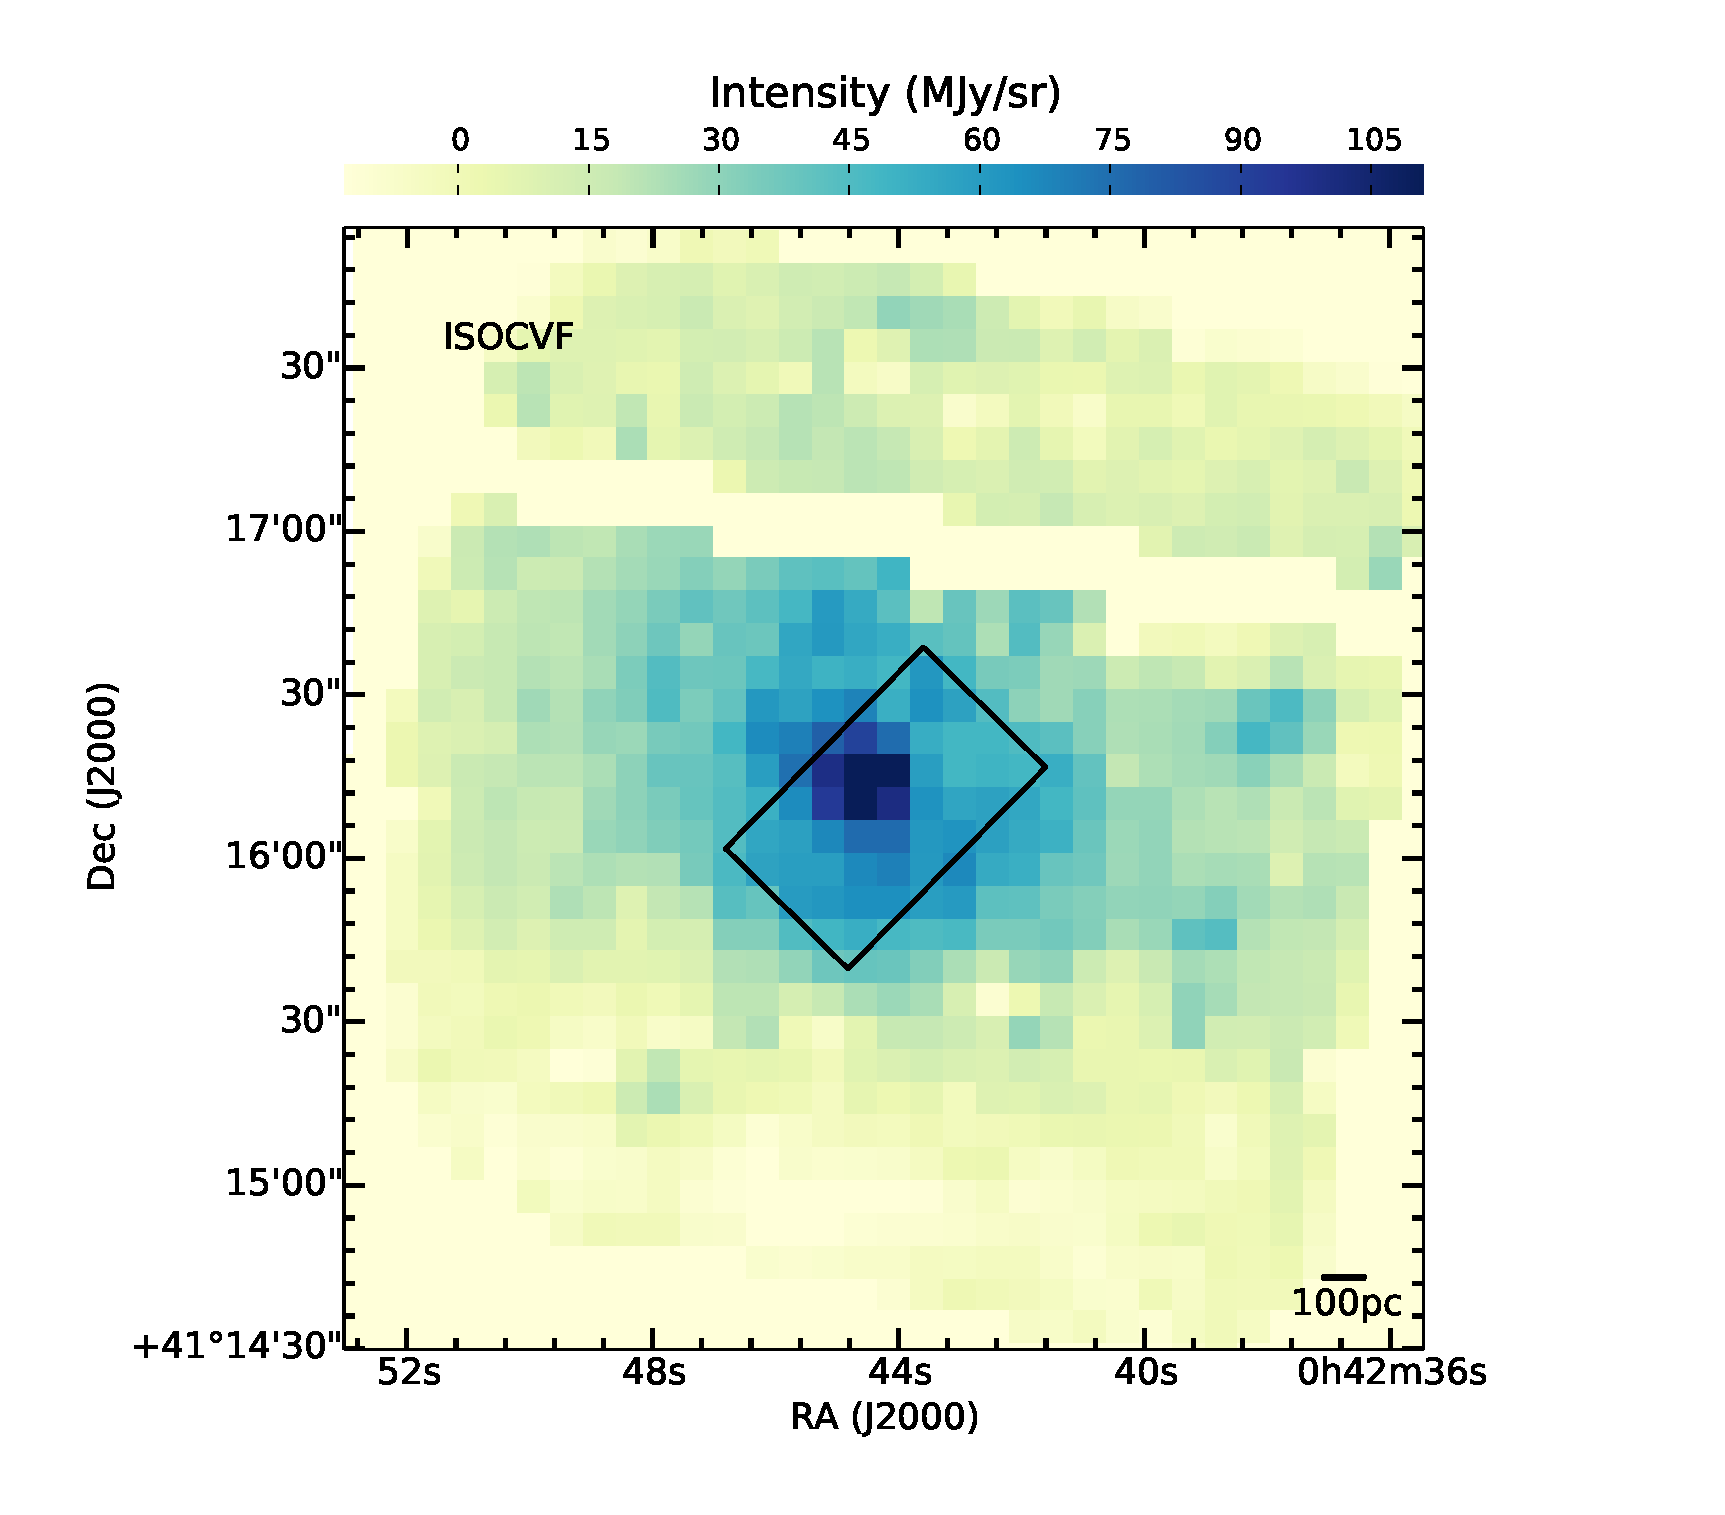
\includegraphics[width = 8cm]{./fig5.eps}
\caption{11.3~$\mu$m negative image (dark colours indicate higher flux) of the ISOCAM data cube from the nucleus of M31. 
The black box shows the size of the aperture ($30\arcsec\times50\arcsec$) used to extract spectra.}
\label{isonuc}
\end{figure}







\section{Spectral characteristics and feature measurements}
\label{sect:data_analysis}


The final processed IRS spectra are shown in  Figure \ref{PAHFITplots}, except for the nucleus, discussed in Section~\ref{sect:nucleus}.
All of the main PAH features, including the 6.2, 7.7, 8.6 and 11.3~$\mu$m bands, 
are clearly visible for all the regions shown here.
The IRS spectra also show atomic line emission such as [Ar~{\sc ii}], [Ar~{\sc iii}], [S~{\sc iii}], [S~{\sc iv}], [Ne~{\sc ii}], [Ne~{\sc iii}] 
and molecular H$_{2}$ emission at 12.3~$\mu$m. Some of the spectra display a contribution to the continuum from starlight emission.


\begin{figure*}
\centering
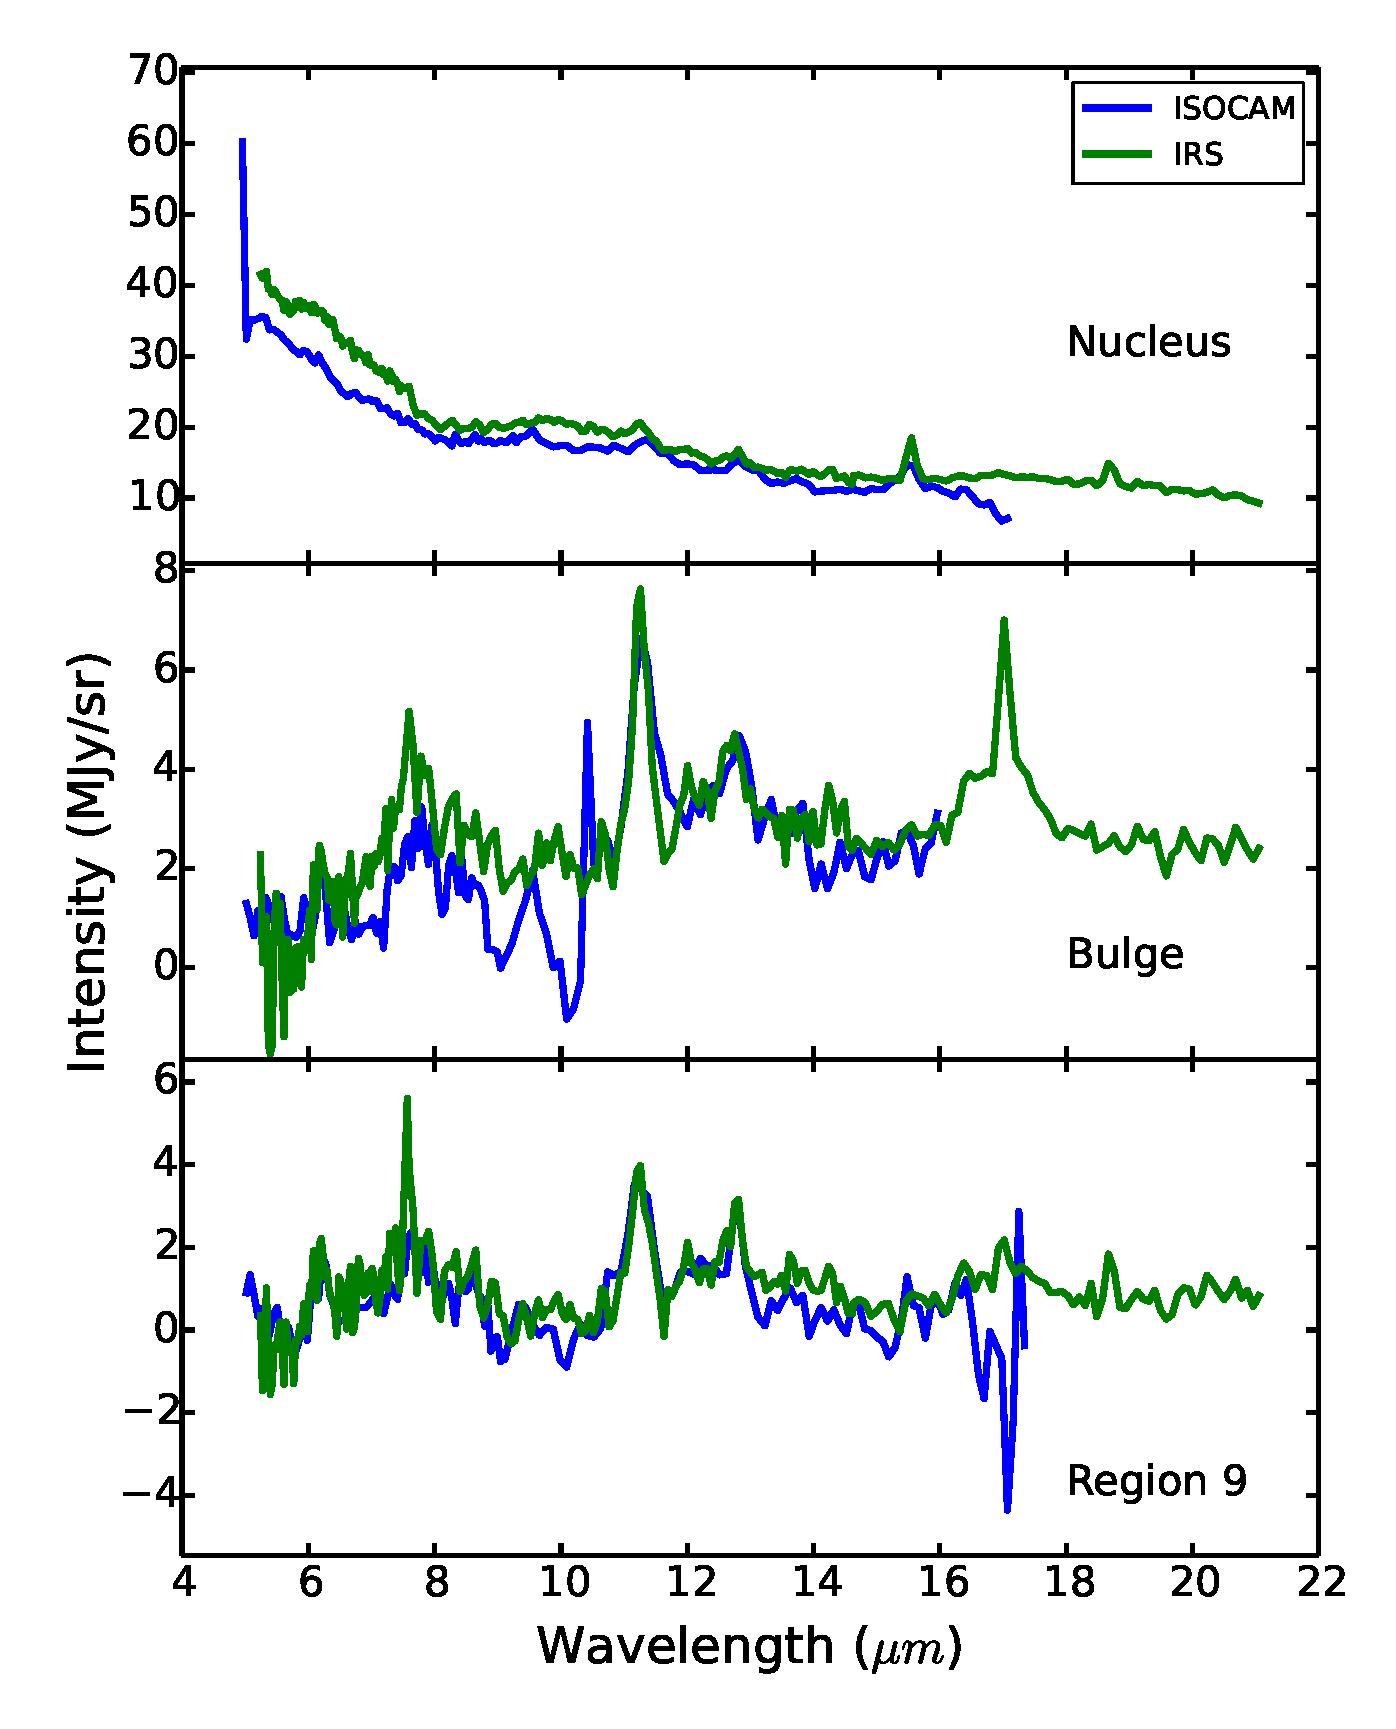
\includegraphics[scale=0.45]{./fig6.eps}
 \caption{Observed IRS spectra and detailed PAHFIT decompositions (see Section~\ref{sect:pahfit}). Regions are labeled in each panel.
Black squares show the observed data, and red, blue, light blue, pink and green lines represent the modelled
dust continua, PAH features, atomic lines, starlight continuum and the fit respectively. The black line shows the total modelled continuum. 
Vertical scales differ in different panels. Spectra from the nucleus and NGC 206 are not shown here.
}
\label{PAHFITplots}
\end{figure*}


\subsection{ISOCAM versus IRS}
\label{sect:iso_vs_irs}

As mentioned in the Introduction, based on ISOCAM observations of four regions in M31, \citet{1998Cesarsky} reported 
suppression of the common 6--8~$\mu$m PAH bands and a strong 11.3$\mu$m PAH band.
The 11.3~$\mu$m band profile was found to vary from region to region.  
In addition, \citet{Pagani_1999} confirmed that the star-forming ring in M31 shows very weak PAH emission in the 6 to 8~$\mu$m region. 
However, the IRS spectra presented here, except the nucleus, do not show such unusual behaviour (Figure~\ref{PAHFITplots}). 
Indeed all regions, except the nucleus, show a normal mid-infrared spectrum similar to other nearby starforming galaxies. 

Until 2005, ISOCAM-CVF data were not properly background subtracted and they were contaminated with zodiacal emission and stray light. 
Differential spectra between regions of relatively strong and weak emission were previously used to overcome this problem 
(more details about the differential spectra are given by \citealt{1998Cesarsky}, \citealt{Pagani_1999}). 
In 2005, all ISOCAM-CVF data were reprocessed  and corrected for the zodiacal emission \citep{Boulanger_F_2005}. 
We obtained newly-processed ISOCAM spectra from three regions in our IRS sample (see Section~\ref{sect:iso_data}) 
in order to compare them with the corresponding IRS spectra.
Figure~\ref{ISOnIRS} shows that although the relative feature intensities  in the IRS and ISOCAM 
spectra differ in detail, the spectral shapes are almost identical;
the re-processed ISOCAM data do not agree with the previous differential spectra.
Neither the bulge nor Region 9 shows any depletion in  6 to 8~$\mu$m features as described by \citet{1998Cesarsky}. 
The new ISOCAM reduction appears to eliminate the discrepancies between ISOCAM and IRS, resulting
in less `strange' infrared spectra for M31. For the remainder of this work, we discuss only the IRS spectra.



\begin{figure}
\centering
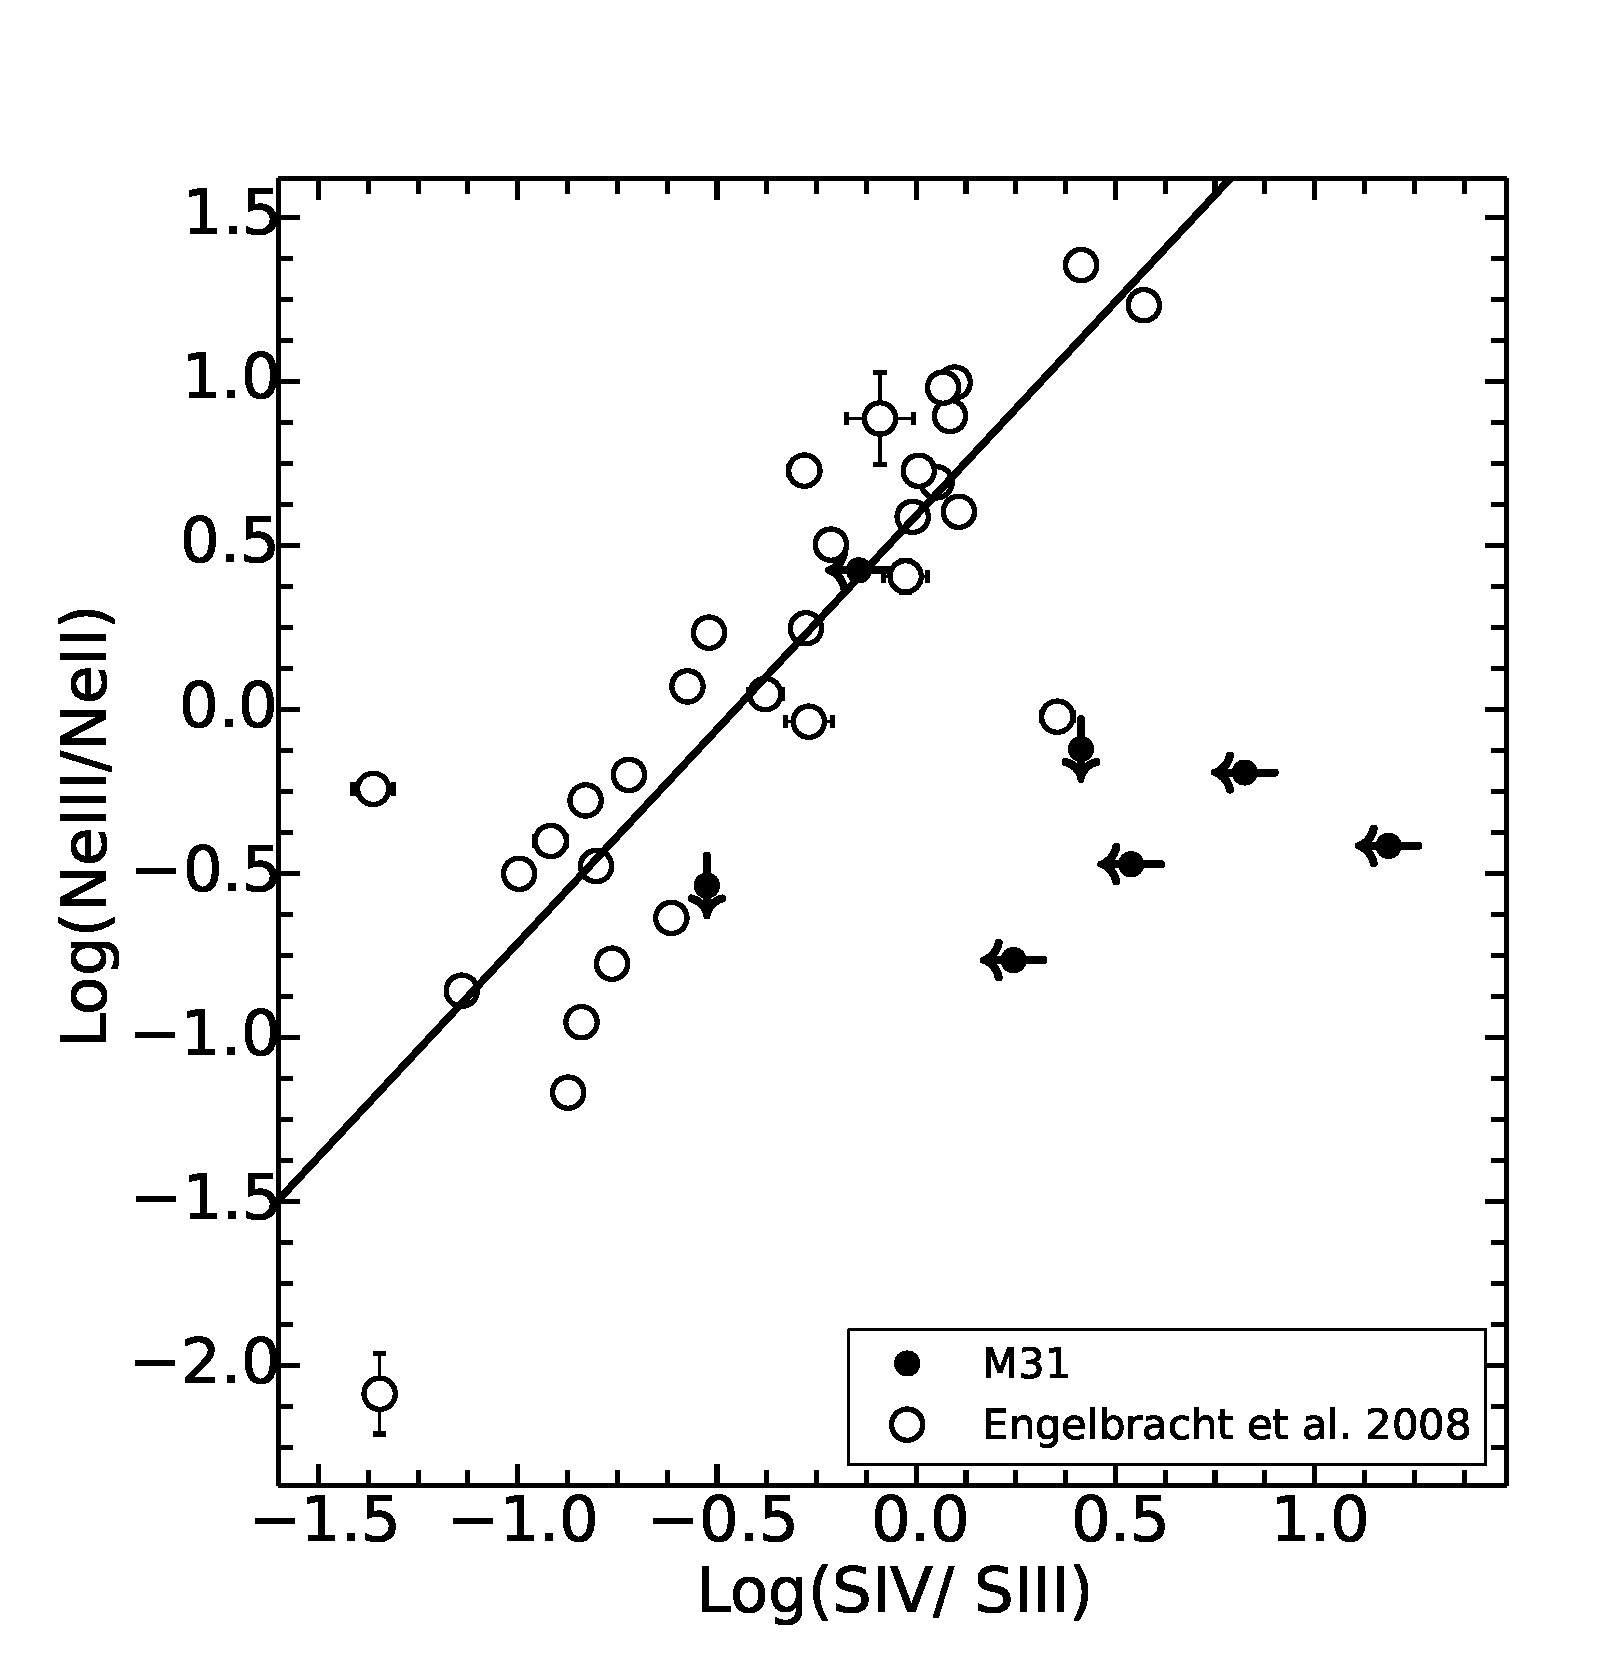
\includegraphics[scale=0.35]{./fig7.eps}
\caption{ Comparison of  IRS and re-processed ISOCAM spectra for the Nucleus (top), Bulge (middle) and Region 9 (bottom) in M31.}
\label{ISOnIRS}
\end{figure}



\subsection{PAHFIT}
\label{sect:pahfit}
The PAH features in  IRS spectra are often blended with neighbouring PAH features and atomic lines. 
Therefore measuring the strength of PAH features is difficult.  To achieve this task a tool called PAHFIT, introduced by \citet{Smith:2007lr}, was used. 
PAHFIT is an IDL  based tool designed for decomposing {\em Spitzer} IRS low-resolution spectra of PAH emission sources.
PAHFIT uses six main components to fit the surface brightness. These are starlight continuum, featureless thermal dust continuum, 
pure rotational lines of H$_2$, fine-structure lines, dust emission features and dust extinction. The starlight is represented by  blackbody 
emission at a fixed temperature of 5000~K, and the dust continuum is represented by 8 modified blackbodies (emissivity proportional to $\nu^2$)  
at fixed temperatures of 35, 40, 50, 65, 90, 135, 200, and 300~K. The final fit obtained with PAHFIT does not necessarily use
all eight dust components.
The infrared extinction is considered as a combination of a power law plus silicate absorption features with peaks at 9.7 and 18~$\mu$m. 
Line features are represented by Gaussian profiles with widths set by the instrumental resolution
and dust features are represented by Drude profiles; more details about PAHFIT are given by \citet{Smith:2007lr}.


Initial attempts at fitting the spectra with PAHFIT showed that some components were negligible, and
to avoid over-fitting we re-ran the fits without these components.
None of the IRS spectra shows significant silicate absorption around 9.7 or 18~$\mu$m, and the extinction calculated by PAHFIT 
was almost zero for all the initial fits. Except for four regions (the bulge, Region 5, Region 6 and Region 8),
the starlight contribution is also negligible.
We adjusted the PAHFIT input parameters to fix extinction to zero for all regions and starlight to zero for all but the four regions above.
Typically only two or three thermal dust components had significant power in our fits, but we did not fix the unused components to zero.
Regions 3 and 9 were found to have very low dust continuum emission compared to other spectra,
possibly because of noisy data at short wavelengths. However the other features in these spectra appear to
be fit correctly. The spectrum of the nucleus shows silicate emission, which is not included in PAHFIT;  
our modifications of PAHFIT to analyze this spectrum are discussed in see Section~\ref{sect:nucleus}.

\begin{table*}
 \centering
 \begin{minipage}{200mm}
\caption{PAH Emission Line Strengths$^a$}
{\scriptsize
  \begin{tabular}{l c c  c  c  c  c  c  c  c  c c }
\hline
    {Region }&{5.7 $\mu$m  }&{6.2 $\mu$m  }&{7.7 $\mu$m$^b$  }&{8.3 $\mu$m  }&{8.6 $\mu$m  }&{10.7 $\mu$m  }&{11.3 $\mu$m$^b$  }&{12.0 $\mu$m  }&{12.7 $\mu$m$^b$  }&{17.0 $\mu$m$^b$  } \\
 \hline

       Bulge  & \dots & $1.32 \pm 0.08$ & $7.7 \pm 0.6$ & $1.1 \pm 0.2$ & $0.7 \pm 0.1$ & $0.07 \pm 0.03$ & $1.85 \pm 0.08$ & $0.49 \pm 0.05$ & $1.02 \pm 0.09$ & $1.39 \pm 0.04$\\
    Region 1  & $0.36 \pm 0.05$ & $1.20 \pm 0.04$ & $3.8 \pm 0.2$ & $0.46 \pm 0.04$ & $0.50 \pm 0.03$ & $0.08 \pm 0.01$ & $1.18 \pm 0.02$ & $0.32 \pm 0.02$ & $0.54 \pm 0.02$ & $0.58 \pm 0.02$\\
    Region 2  & $0.27 \pm 0.03$ & $1.10 \pm 0.03$ & $3.7 \pm 0.2$ & $0.33 \pm 0.04$ & $0.70 \pm 0.03$ & $0.053 \pm 0.008$ & $1.13 \pm 0.02$ & $0.23 \pm 0.01$ & $0.51 \pm 0.03$ & $0.51 \pm 0.02$\\
    Region 3  & $0.3 \pm 0.1$ & $0.9 \pm 0.1$ & $3.9 \pm 0.6$ & $0.7 \pm 0.1$ & $0.3 \pm 0.1$ & \dots & $0.68 \pm 0.07$ & $0.21 \pm 0.05$ & $0.47 \pm 0.07$ & $0.45 \pm 0.04$\\
    Region 4  & $0.14 \pm 0.04$ & $0.56 \pm 0.03$ & $2.1 \pm 0.2$ & $0.26 \pm 0.04$ & $0.41 \pm 0.03$ & $0.029 \pm 0.008$ & $0.70 \pm 0.02$ & $0.12 \pm 0.01$ & $0.31 \pm 0.02$ & $0.44 \pm 0.02$\\
    Region 5  & \dots & $0.24 \pm 0.04$ & $0.79 \pm 0.07$ & $0.12 \pm 0.04$ & $0.21 \pm 0.03$ & $0.032 \pm 0.008$ & $0.45 \pm 0.02$ & $0.09 \pm 0.01$ & $0.22 \pm 0.01$ & $0.33 \pm 0.04$\\
    Region 6  & \dots & $0.26 \pm 0.03$ & $0.8 \pm 0.2$ & $0.10 \pm 0.03$ & $0.13 \pm 0.03$ & $0.029 \pm 0.008$ & $0.38 \pm 0.02$ & $0.07 \pm 0.01$ & $0.16 \pm 0.01$ & $0.29 \pm 0.02$\\
    Region 7  & $0.21 \pm 0.03$ & $0.62 \pm 0.03$ & $2.0 \pm 0.2$ & $0.30 \pm 0.04$ & $0.45 \pm 0.03$ & $0.058 \pm 0.008$ & $0.77 \pm 0.02$ & $0.18 \pm 0.01$ & $0.37 \pm 0.03$ & $0.47 \pm 0.04$\\
    Region 8  & \dots & $0.09 \pm 0.04$ & $0.22 \pm 0.07$ & $0.09 \pm 0.04$ & $0.10 \pm 0.03$ & $0.051 \pm 0.009$ & $0.16 \pm 0.02$ & \dots & \dots & $0.15 \pm 0.02$\\
    Region 9  & \dots & $1.3 \pm 0.1$ & $4.4 \pm 0.6$ & $0.9 \pm 0.1$ & $0.5 \pm 0.1$ & $0.09 \pm 0.03$ & $1.32 \pm 0.07$ & $0.51 \pm 0.05$ & $0.83 \pm 0.07$ & $0.6 \pm 0.1$\\

 \hline
 \label{PAHlinetable}
\end{tabular}\\
{$^a$Units are 10$^{-15}$~W~m$^{-2}$.\\
$^b$PAH complexes, as described in text.}
}
\end{minipage}
\end{table*}



\begin{table*}
 \centering
 \begin{minipage}{200mm}
 
\caption{PAH Emission Line Equivalent Widths$^a$}
 {\scriptsize
  \begin{tabular}{l c c  c  c  c  c  c  c  c  c c }
  \hline 
     {Region }&{5.7 $\mu$m  }&{6.2 $\mu$m  }&{7.7 $\mu$m$^b$  }&{8.3 $\mu$m  }&{8.6 $\mu$m  }&{10.7 $\mu$m  }&{11.3 $\mu$m$^b$  }&{12.0 $\mu$m  }&{12.7 $\mu$m$^b$  }&{17.0 $\mu$m$^b$  } \\
 \hline
       Bulge  & \dots & $1.2 \pm 0.2$ & $4.1 \pm 0.4$ & $0.51 \pm 0.07$ & $0.30 \pm 0.06$ & $0.03 \pm 0.01$ & $0.78 \pm 0.04$ & $0.22 \pm 0.02$ & $0.49 \pm 0.05$ & $1.16 \pm 0.04$\\
    Region 1  & $0.39 \pm 0.08$ & $1.2 \pm 0.1$ & $3.4 \pm 0.3$ & $0.43 \pm 0.04$ & $0.47 \pm 0.04$ & $0.09 \pm 0.01$ & $1.45 \pm 0.04$ & $0.43 \pm 0.03$ & $0.76 \pm 0.04$ & $1.26 \pm 0.05$\\
    Region 2  & $0.28 \pm 0.04$ & $1.02 \pm 0.06$ & $3.4 \pm 0.2$ & $0.32 \pm 0.04$ & $0.70 \pm 0.04$ & $0.07 \pm 0.01$ & $1.58 \pm 0.04$ & $0.35 \pm 0.02$ & $0.85 \pm 0.05$ & $1.33 \pm 0.06$\\
    Region 3  & $4.3 \pm 2.3$ & $8.3 \pm 2.3$ & $18.5 \pm 4.2$ & $2.8 \pm 0.8$ & $0.9 \pm 0.5$ & \dots & $2.1 \pm 0.3$ & $0.7 \pm 0.2$ & $1.6 \pm 0.3$ & $2.4 \pm 0.3$\\
    Region 4  & $0.28 \pm 0.09$ & $1.0 \pm 0.1$ & $3.7 \pm 0.4$ & $0.48 \pm 0.07$ & $0.77 \pm 0.07$ & $0.07 \pm 0.02$ & $1.67 \pm 0.06$ & $0.31 \pm 0.04$ & $0.82 \pm 0.06$ & $1.65 \pm 0.08$\\
    Region 5  & \dots & $0.12 \pm 0.03$ & $0.61 \pm 0.07$ & $0.10 \pm 0.03$ & $0.20 \pm 0.03$ & $0.05 \pm 0.01$ & $0.77 \pm 0.04$ & $0.17 \pm 0.03$ & $0.50 \pm 0.04$ & $1.6 \pm 0.2$\\
    Region 6  & \dots & $0.10 \pm 0.04$ & $0.6 \pm 0.2$ & $0.10 \pm 0.04$ & $0.14 \pm 0.03$ & $0.05 \pm 0.01$ & $0.77 \pm 0.05$ & $0.15 \pm 0.03$ & $0.42 \pm 0.05$ & $1.7 \pm 0.1$\\
    Region 7  & $0.32 \pm 0.05$ & $0.86 \pm 0.06$ & $2.2 \pm 0.1$ & $0.44 \pm 0.06$ & $0.69 \pm 0.06$ & $0.12 \pm 0.02$ & $1.81 \pm 0.07$ & $0.48 \pm 0.05$ & $1.08 \pm 0.09$ & $2.2 \pm 0.3$\\
    Region 8  & \dots & \dots & $0.10 \pm 0.05$ & $0.09 \pm 0.04$ & $0.10 \pm 0.03$ & $0.09 \pm 0.02$ & $0.30 \pm 0.04$ & \dots & \dots & $0.62 \pm 0.08$\\
    Region 9  & \dots & $\left(2.4 \pm 1.1\right) \times 10^{2}$ & $\left(1.4 \pm 0.4\right) \times 10^{2}$ & $15.5 \pm 5.6$ & $7.9 \pm 2.8$ & $0.5 \pm 0.2$ & $6.8 \pm 1.1$ & $2.3 \pm 0.6$ & $3.5 \pm 0.8$ & $2.2 \pm 0.8$\\

 \hline
 \label{EQW}
\end{tabular}\\
{$^a$Units are $\mu$m.\\
$^b$PAH complexes, as described in text.\\
Continuum for Regions 3 and 9 is very weak.  Equivalent widths are highly uncertain and not considered in the analysis (see Section~\ref{sect:data_analysis}).}
}
\end{minipage}
\end{table*}



\subsection{PAH features}
\label{sect:pah}

PAHFIT returns fluxes and equivalent widths (EQWs) of PAH features, which are given in Tables~\ref{PAHlinetable} and \ref{EQW}. 
For easier comparison with previous work, the tables give measurements for the 7.7, 11.3, 12.7 and 17.0~$\mu$m PAH complexes
as defined by \citet{Smith:2007lr}, as computed from the individual constituent features measured by PAHFIT.
The intensities of the features do not include any contribution from the continuum, but the equivalent width computed by
\begin{equation}
{\rm EQW}=\int \frac{I_{\nu,{\rm feature}}}{I_{\nu, {\rm cont}}} \,d\lambda,
\end{equation}
is a measure of the ratio of the continuum emission ($I_{\nu, {\rm cont}} $) to the line strength 
($I_{\nu,{\rm feature}}=I_{\nu} =- I_{\nu, {\rm cont}})$. 
The continuum emission is mainly from dust grains, much larger than PAH molecules. Hence, by studying EQWs of PAHs, 
we can study how the PAHs compete with the dust grains in the mid-infrared wavelengths.  PAHFIT returns the EQWs for each PAH 
feature, we calculated the uncertainties using a Monte-Carlo method. In that method, for each region, PAHFIT was run 500 times on 
randomly generated data points  normally distributed within the uncertainties of the spectrum. PAHFIT returned 500 EQWs for each 
PAH feature, and the standard deviation of EQWs for a given feature was taken as its uncertainty. 
The EQWs from Regions 3 and 9 were removed from further analysis because the negligible dust continuum for these spectra makes
the EQWs highly uncertain.


\subsection{Atomic line features}
\label{sect:atomic}


\begin{figure}
\centering
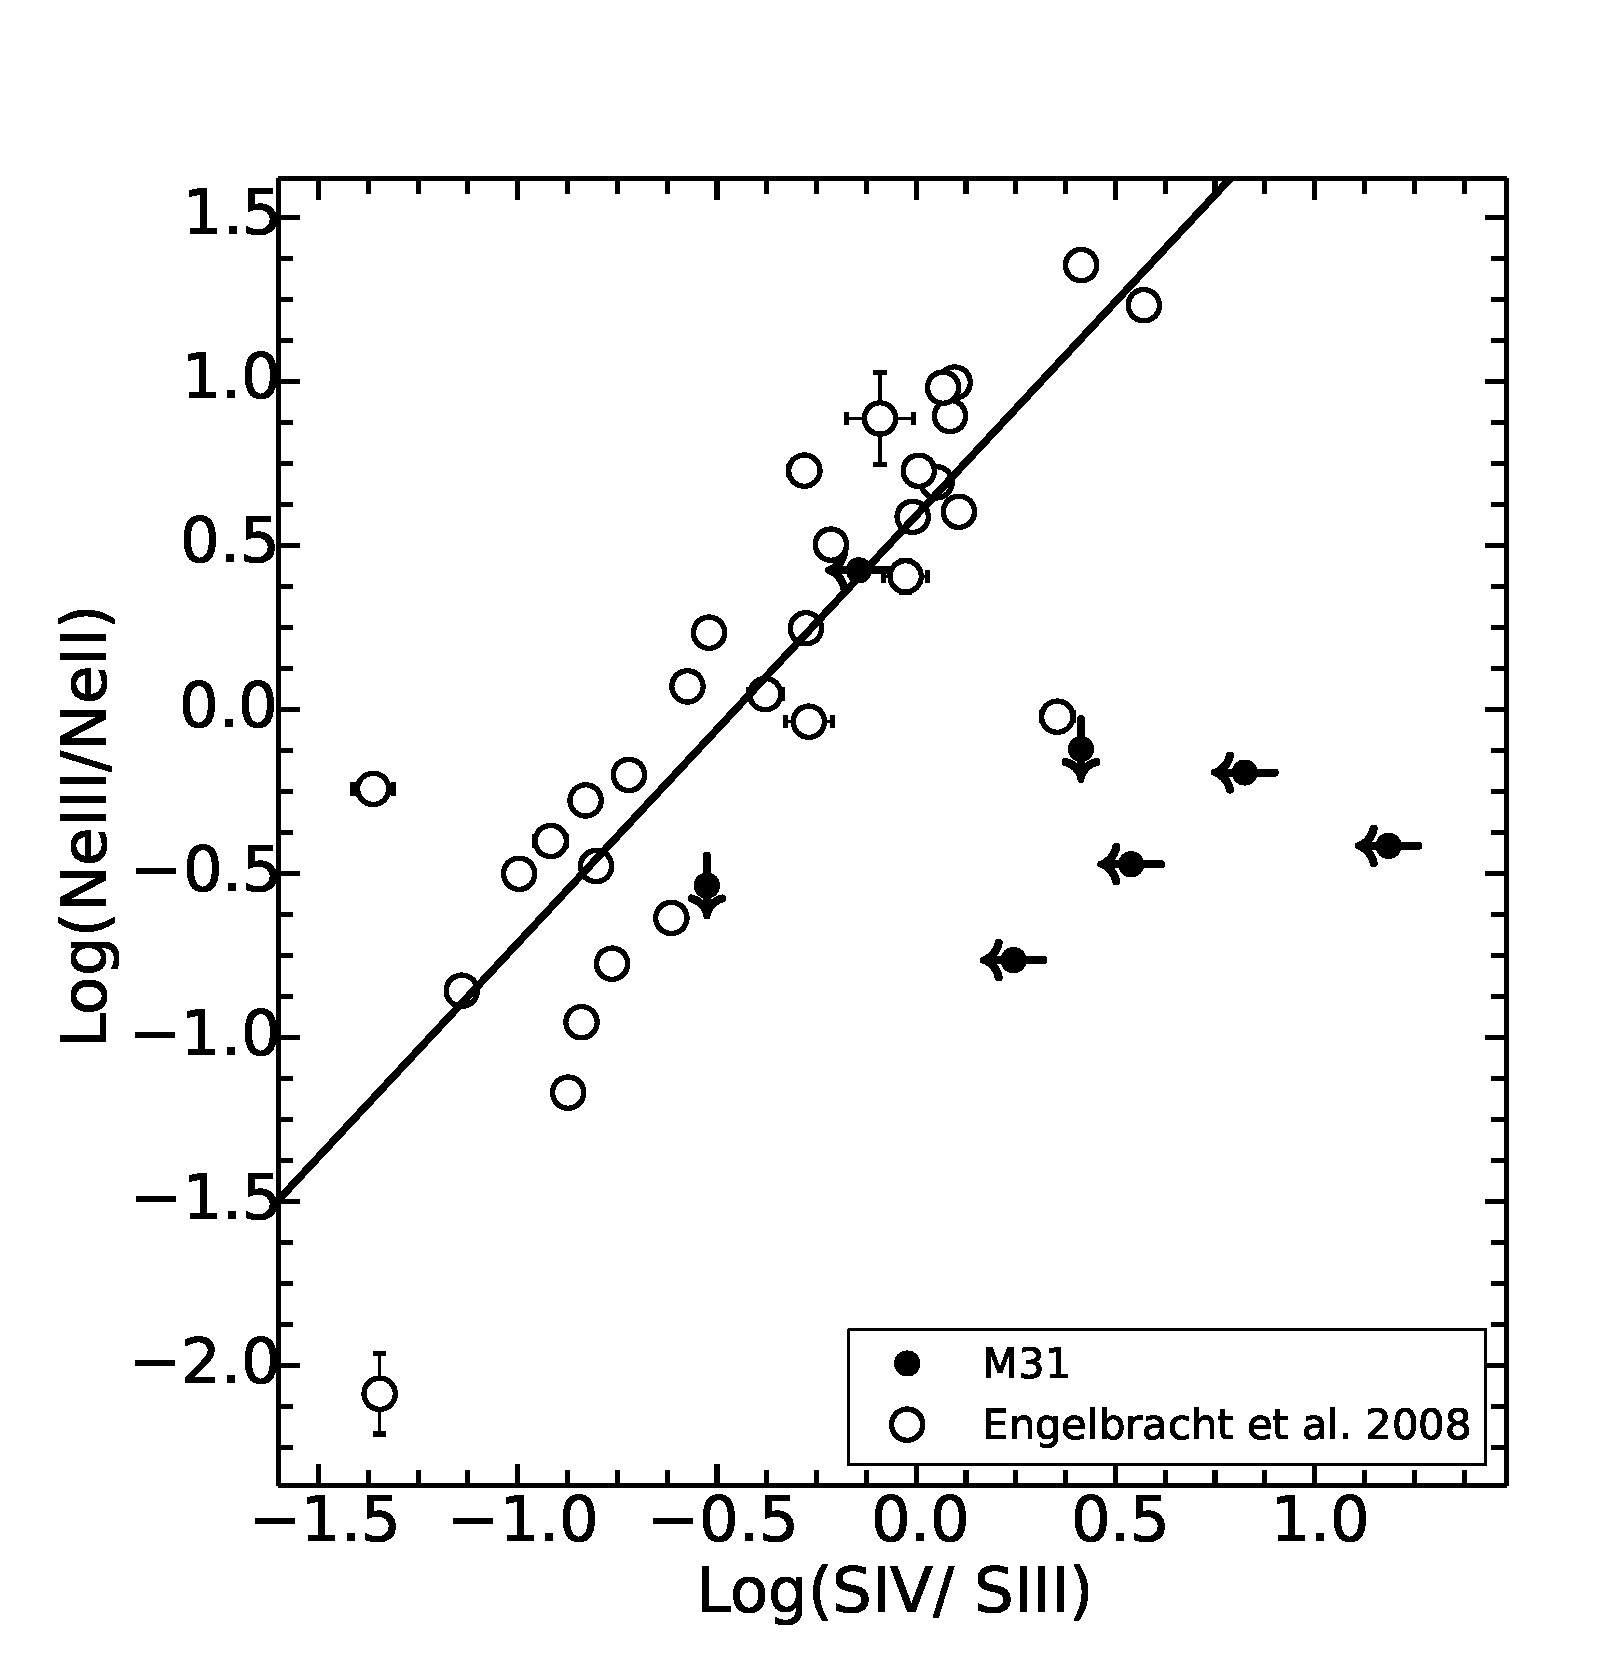
\includegraphics[scale=0.3]{./fig8.eps}
\caption{ Log([Ne~{\sc iii}]/[Ne~{\sc ii}])  vs log([S~{\sc iv}]/[S~{\sc iii}])  for the M31 regions in our sample (black dots) and  the starburst sample from \citet{Engelbracht_2008} (open dots). The straight line is the line of best fit for the starburst sample.
Upper limits are $3\sigma$.
}
\label{SvsNe}
\end{figure}

PAHFIT also returns the line strengths and uncertainties for atomic lines, listed in Table~\ref{Atomic}.
Not all lines were detected by PAHFIT, so we calculated upper limits for non-detected lines.%
\footnote{To find  the upper limits for the flux of missing atomic lines, we assumed the line to be a 
Gaussian profile with a FWHM as given by PAHFIT. The peak intensity was taken to be 3 times the RMS, where RMS is the root mean square of 
the noise at the position of a missing line.}
Line ratios of [Ne~{\sc iii}]/[Ne~{\sc ii}] and [S~{\sc iv}]/[S~{\sc iii}]~18 have been used as an indication of the radiation hardness, and
\citet{Engelbracht_2008} defined a combination of these two line ratios as a 'radiation hardness index (RHI)':
\begin{equation}
{\rm RHI} = \left( \log\frac{\textrm{[Ne~{\sc iii}] }}{\textrm{[Ne~{\sc ii}]}} + \left[0.71 + 1.58\log\frac{\textrm{{[S~{\sc iv}]}}}{\textrm{{[S~{\sc iii}]}}}\right]\right) /2
\end{equation}
\label{eq:rhi}
Here, 1.58 and 0.71 are the slope and intercept of the [Ne~{\sc iii}]/[Ne~{\sc ii}]  vs [S~{\sc iv}]/[S~{\sc iii}] plot (Figure \ref{SvsNe}) for the starburst sample from 
\citet{Engelbracht_2008}. The RHI has also been used by \citet{Gordon:2008lr} for M101 observations. 
Figure \ref{SvsNe}  compares the atomic line emission from the selected regions of M31 to the starburst galaxy sample;
although none of our spectra have detections of all four lines, our limits are mostly consistent with the wtrend.
We therefore compute the RHI using the first term of equation~\ref{eq:rhi} for the regions with missing S lines
and the second term for the regions with missing Ne lines.
Regions 2, 5, and 8 had detections of only one line per element, so we used the appropriate upper limits 
to calculate RHI for these spectra.


\begin{table*}
 \centering
 \begin{minipage}{100mm}
\caption{Atomic Emission Line Strengths$^a$}
  \begin{tabular}{l c c  c  c  c  c  }
  \hline
  {Region  }&{[Ar~{\sc ii}] }&{[Ar~{\sc iii}]  }&{[S~{\sc iv}]}&{[Ne~{\sc ii}]   }&{[Ne~{\sc iii}]   }&{[S~{\sc iii}]  }\\
{}&{\tiny{7.0 $\mu$m} }&{\tiny{9.0 $\mu$m }}&{\tiny{10.5 $\mu$m}}&{\tiny{12.8 $\mu$m  }}&{\tiny{15.5 $\mu$m } }&{\tiny{18.7 $\mu$m }} \\
 \hline 
       Bulge  & $<0.12$ & $0.17 \pm 0.03$ & $<0.11$ & $0.07 \pm 0.01$ & $0.025 \pm 0.006$ & $0.007 \pm 0.003$\\
    Region 1  & $<0.05$ & $<0.06$ & $0.020 \pm 0.004$ & $0.020 \pm 0.004$ & $<0.01$ & $0.008 \pm 0.001$\\
    Region 2  & $<0.05$ & $<0.06$ & $<0.02$ & $0.022 \pm 0.004$ & $<0.01$ & $0.003 \pm 0.002$\\
    Region 3  & $<0.15$ & $0.09 \pm 0.02$ & $<0.10$ & $0.03 \pm 0.01$ & $0.020 \pm 0.004$ & $0.015 \pm 0.003$\\
    Region 4  & $<0.04$ & $<0.04$ & $<0.02$ & $<0.02$ & $<0.01$ & $0.004 \pm 0.002$\\
    Region 5  & $<0.04$ & $<0.02$ & $<0.02$ & $<0.01$ & $0.009 \pm 0.004$ & $0.008 \pm 0.004$\\
    Region 6  & $0.02 \pm 0.01$ & $0.014 \pm 0.007$ & $<0.01$ & $<0.01$ & $0.019 \pm 0.002$ & $0.019 \pm 0.002$\\
    Region 7  & $<0.04$ & $<0.04$ & $0.008 \pm 0.003$ & $0.035 \pm 0.005$ & $<0.01$ & $0.027 \pm 0.004$\\
    Region 8  & $<0.04$ & $0.017 \pm 0.006$ & $<0.02$ & $<0.01$ & $0.041 \pm 0.002$ & $0.023 \pm 0.002$\\
    Region 9  & $0.09 \pm 0.04$ & $0.12 \pm 0.03$ & $<0.09$ & $0.13 \pm 0.01$ & $<0.04$ & $0.05 \pm 0.02$\\
\hline
 \label{Atomic}
\end{tabular}\\
{ $^a$Units are 10$^{-15}$~W~m$^{-2}$. Upper limits ($3\sigma$) are indicated with a $<$ mark.  }
\end{minipage}
\end{table*}



\section{Results and discussion}

\subsection{PAH intensities}
\label{sect:pah_ratios}

Both the 6.2 and 7.7~$\mu$m features are thought to be coming from ionized PAHs and the 11.3~$\mu$m feature from neutral PAHs. Therefore we expect to see a correlation between the intensities of 6.2 and 7.7~$\mu$m PAH features normalized by the 11.3~$\mu$m feature.  Figure \ref{PAHlines}  compares the PAH flux ratios of 7.7/11.3  and 6.2/11.3 features. The figure shows a good correlation between these two PAH line ratios, consistent with that of the SINGS sample shown by \citet{Smith:2007lr}.
A similar correlation was also reported by  \citet{Galliano2008} for a sample of galaxies and a handful of extended H{\sc ii} regions
and by \citet{Vermeij2002} for Galactic and Magellanic Cloud {\sc ii}regions. This provides evidence that the PAH emission from M31 is not unusual. 


\begin{figure}
\centering
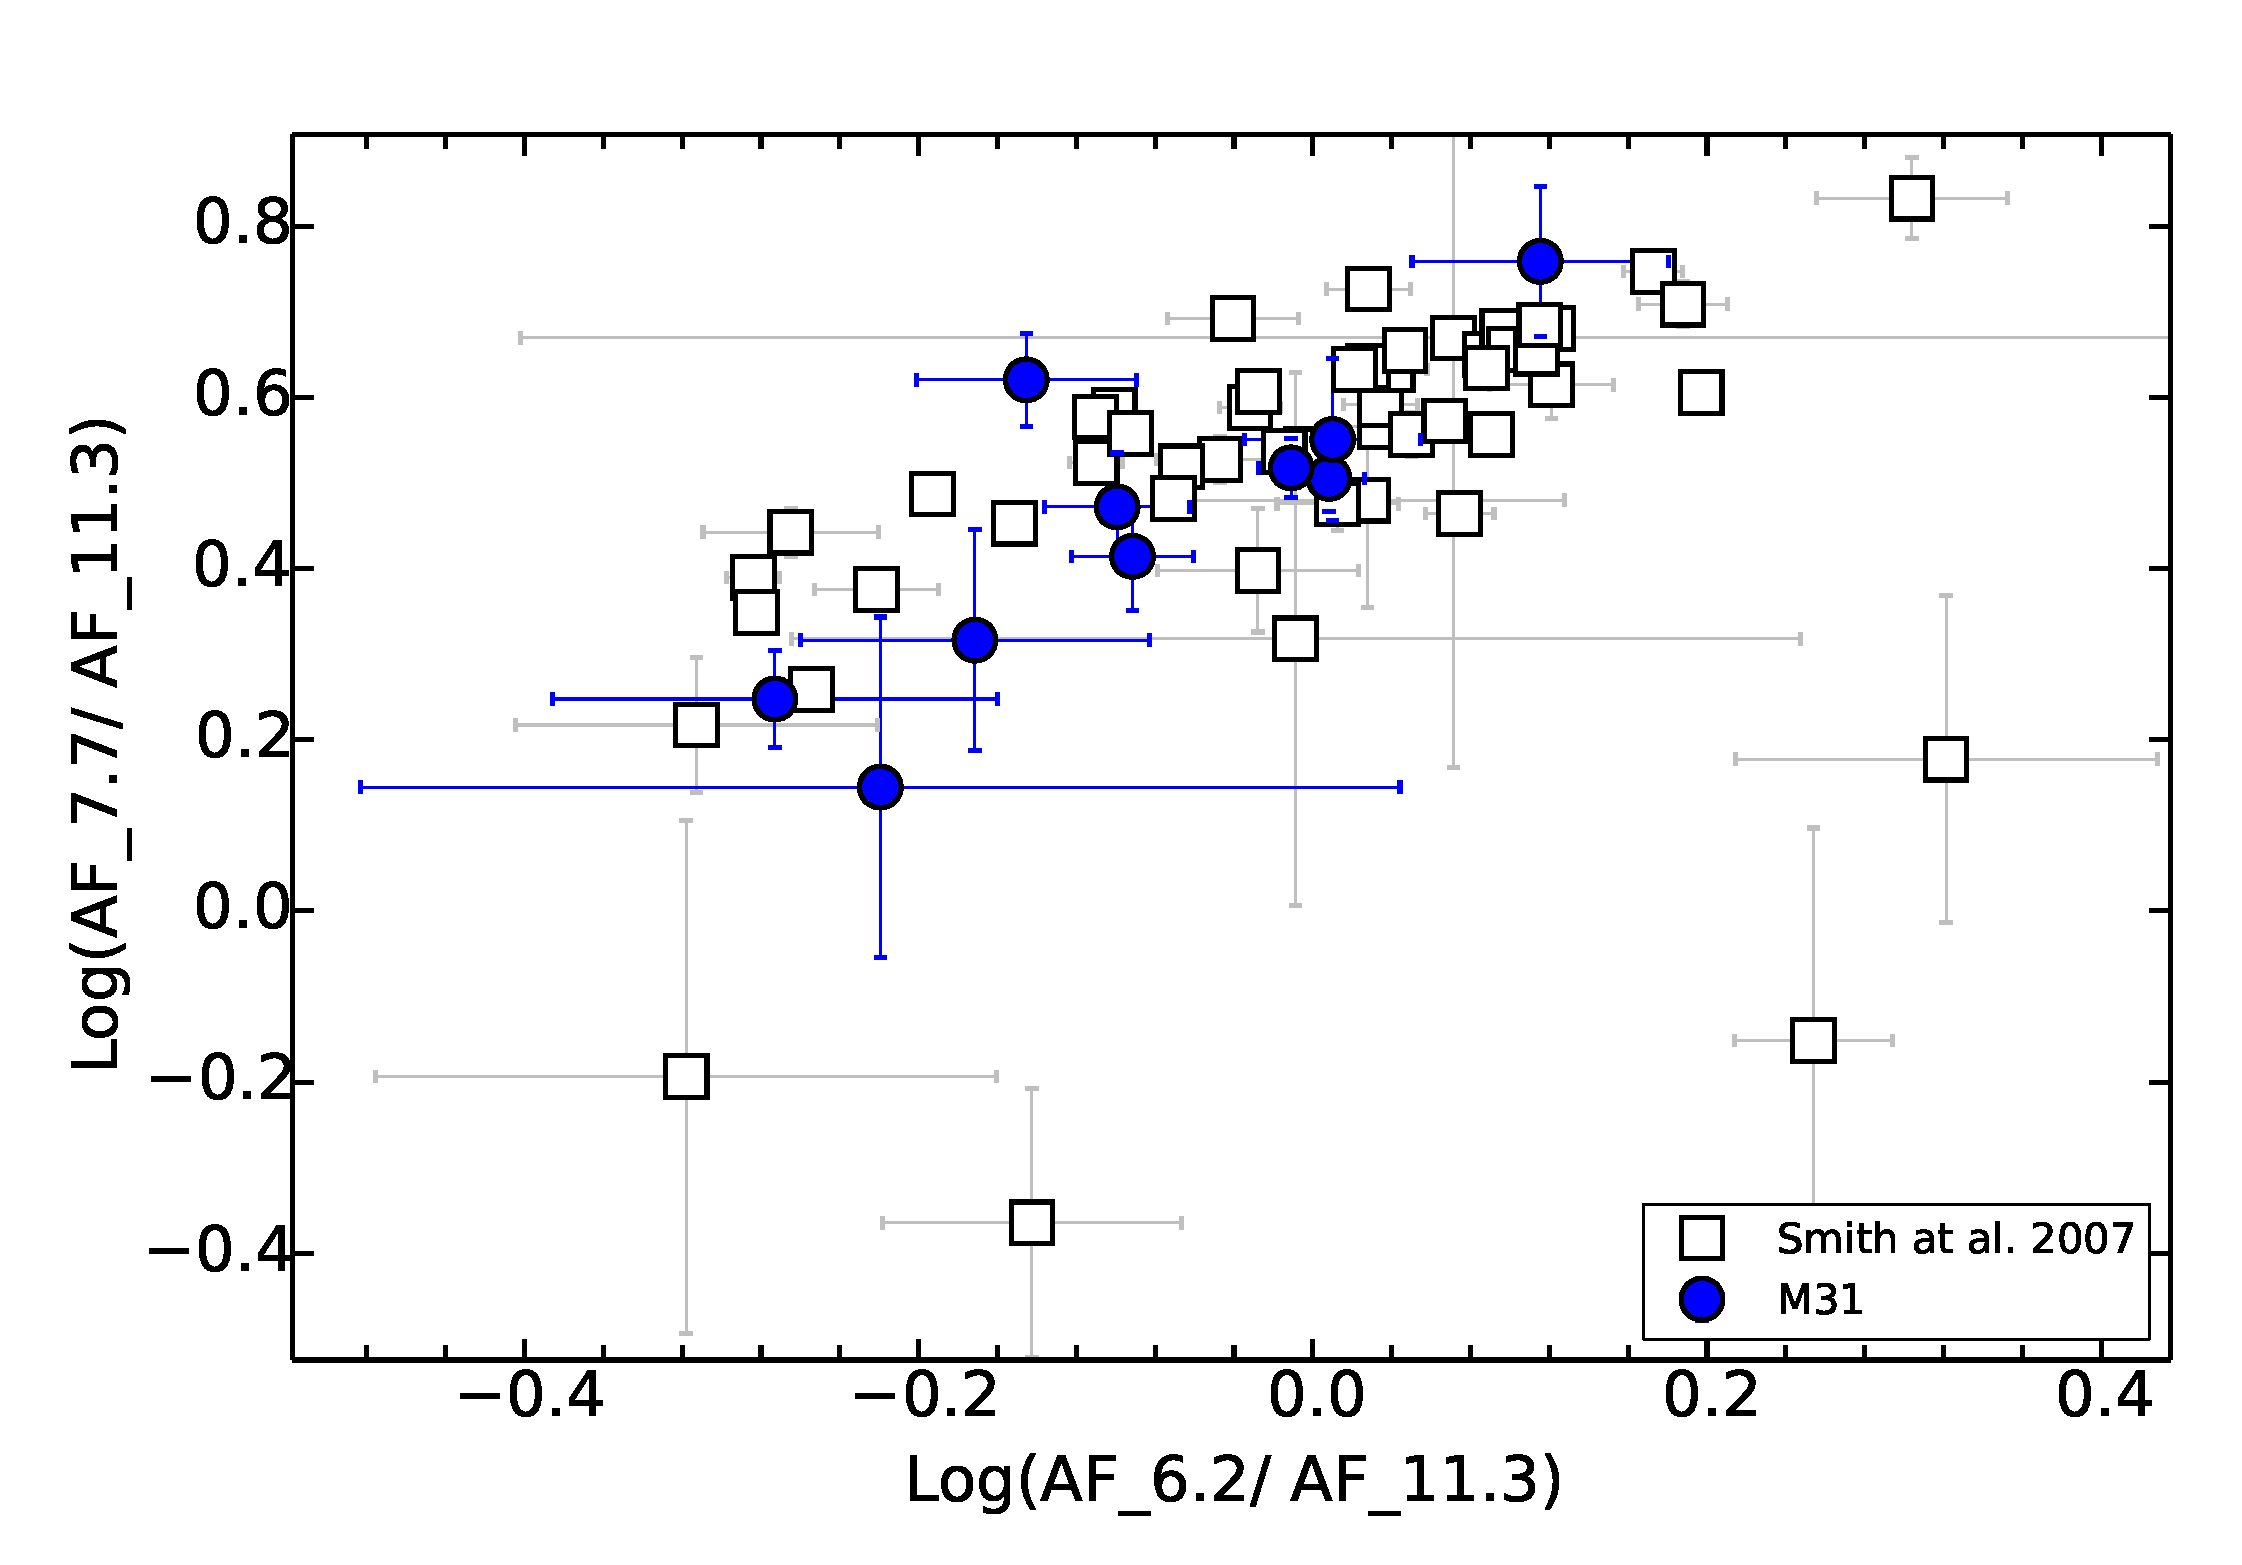
\includegraphics[scale = 0.25]{./fig9.eps}
\caption{Ratios of PAH feature fluxes (7.7~$\mu$m/11.3~$\mu$m versus 6.2~$\mu$m/11.3~$\mu$m) for 10 regions in M31.
Open squares represent the central regions of nearby galaxies as observed in the SINGS sample by \citet{Smith:2007lr}.
}
\label{PAHlines}
\end{figure}

\subsection{PAH equivalent widths versus radiation hardness}
\label{sect:eqw_rh}


\begin{figure}
\centering
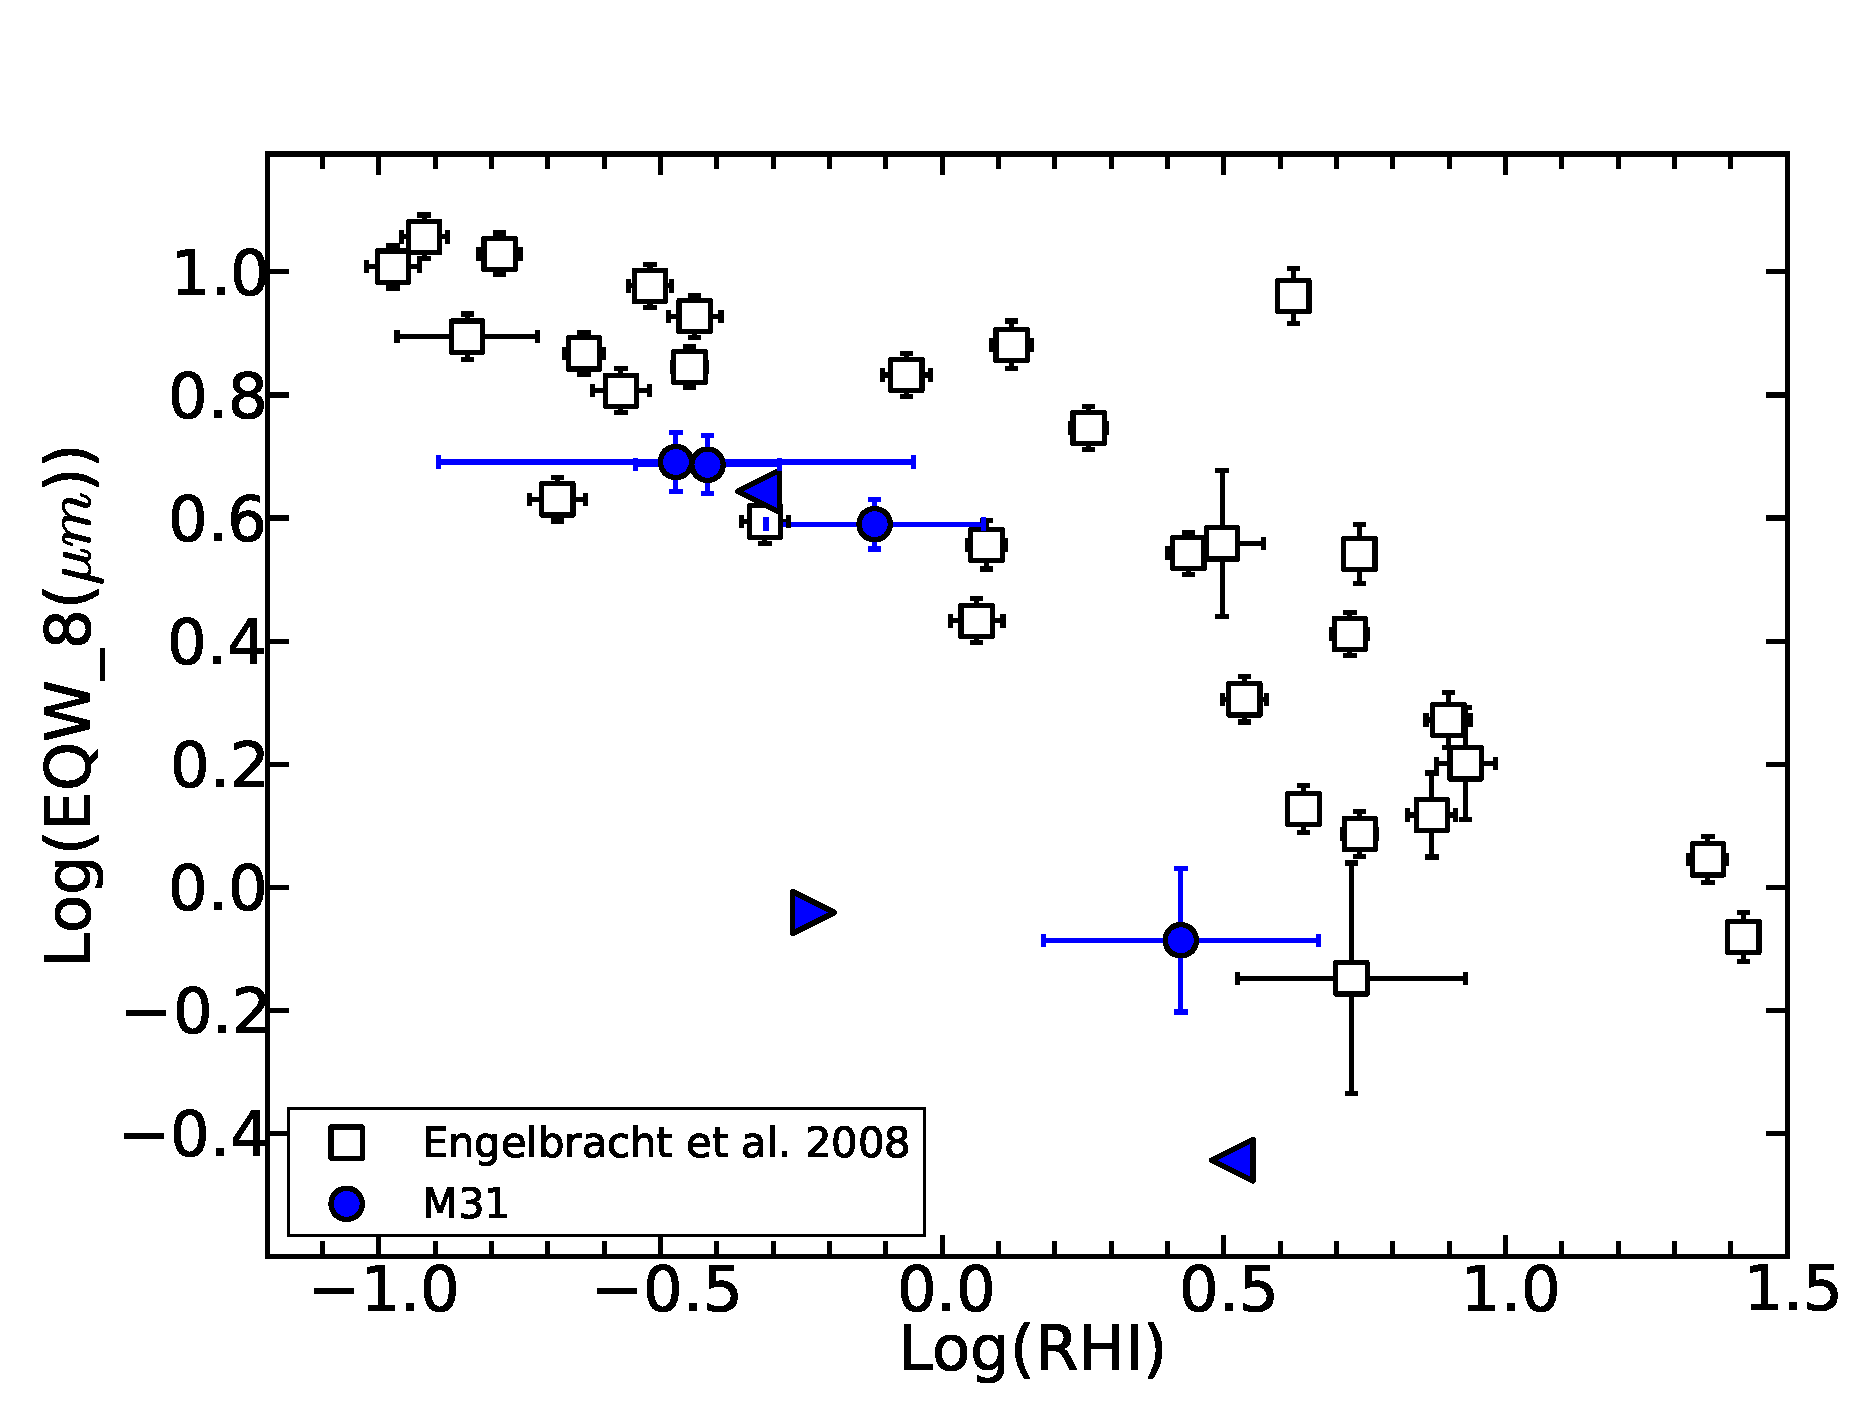
\includegraphics[scale=0.25]{./fig10.eps}
\caption{Equivalent width of the 8~$\mu$m PAH feature versus radiation hardness index (RHI) for the M31 sample (blue). 
The 8~$\mu$m feature is a combination of the 7.7, 8.3 and 8.6~$\mu$m PAHFIT components. 
Open squares represent the starburst galaxy sample from \citet{Engelbracht_2008}, which includes 66 nearby ($2<d<250$~Mpc)
star-bursting or star-forming galaxies selected to cover a wide range in metallicity ($7.1<12+\log{\rm[O/H]}<8.9$).
 For M31 spectra with undetected lines, triangles represent $3\sigma$ upper (left-pointing triangles) and lower (right-pointing triangles)  limits.} 
\label{englII}
\end{figure}

\begin{figure}
\centering
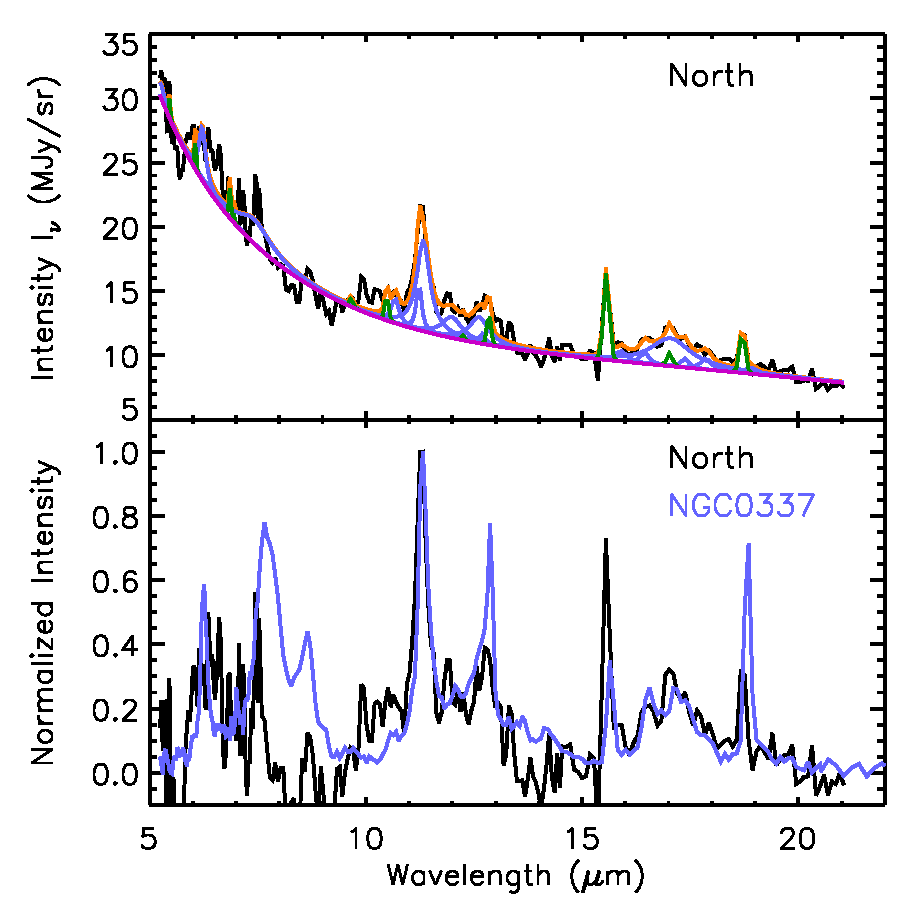
\includegraphics[scale=0.30]{./fig11.eps}
\caption{Equivalent widths of the normalized 7.7~$\mu$m PAH feature (top panel) and 11.3~$\mu$m PAH feature (bottom panel) versus 
radiation hardness index (RHI) for the M31 sample. Open squares represent the seven H~{\sc ii} regions in M101 observed  by \citet{Gordon:2008lr},  
which have $8.1<12+\log{\rm[O/H]}<8.8$ 
The normalization was done by dividing each EQW by the weighted average over all regions in the respective samples. 
Triangles represent $3\sigma$ upper and lower limits.} 
\label{gordII}
\end{figure}


As mentioned in the introduction, PAH equivalent widths tend to show an inverse correlation with radiation hardness. 
The equivalent widths of the M31 PAH features are compared with RHI in Figures~\ref{englII} and \ref{gordII}.
For reference, we also show the starburst sample of \citet{Engelbracht_2008} 
and the seven H~{\sc ii} regions in M101 observed by \citet{Gordon:2008lr}.
To make a direct comparison with the M101 sample, we normalized the M31 EQWs in Figure~\ref{gordII} using the same procedure
as \citet{Gordon:2008lr}, dividing each EQW by the  weighted average over all regions in the respective samples. 
The equivalent widths seem to be decreasing with increasing radiation hardness, consistent with previous results. 
This also helps to confirm that the PAH emission in M31 is not unusual. 


\subsection{PAH equivalent widths versus metallicity}
\label{sect:eqw_met}

Many studies based on ISO and {\em Spitzer} observations have reported that PAH intensity decreases with decreasing metallicity \citep{Calzetti:2010fk}. 
In addition, these studies also report a sudden drop of EQWs of PAHs around $12+\log{\rm (O/H)} \approx 8.1$. 
This has been observed amongst different galaxies \citep{Engelbracht_2008} as well as within a single galaxy \citep{Gordon:2008lr}. 

\citet{Sanders_2011}  measured spectroscopic metallicities for
more than 250 H~{\sc ii} regions using strong line diagnostics.\footnote{\citet{Sanders_2011} considered several different
calibrations for abundance diagnostics. We use the results from the method they denote ``N06 N2''  \citep{Nagao2006} because
that method has the largest sample size.} Except for regions 5 and 8, all of our mapped regions contain an  H~{\sc ii} region measured by
 \citet{Sanders_2011}, and we give the corresponding metallicities in Table~\ref{regions}.
 For regions 5 and 8 we adopted metallicities from the radial metallicity profile of M31 given by
 \citet{Sanders_2011}. It is well known that there are systematic differences between different 
 methods used to measure metallicities, and those in the sample of \citet{Engelbracht_2008} 
 were obtained by the direct electron temperature method  \citep{Skillman1998}.
\citet{Mitchel2014} calculated the offset between direct and strong-line measurements for M31 H~{\sc ii} regions to be 
$0.35\pm0.10$ and we correct for this in Figure~\ref{metalicityVseqw}.

\begin{figure}
\centering
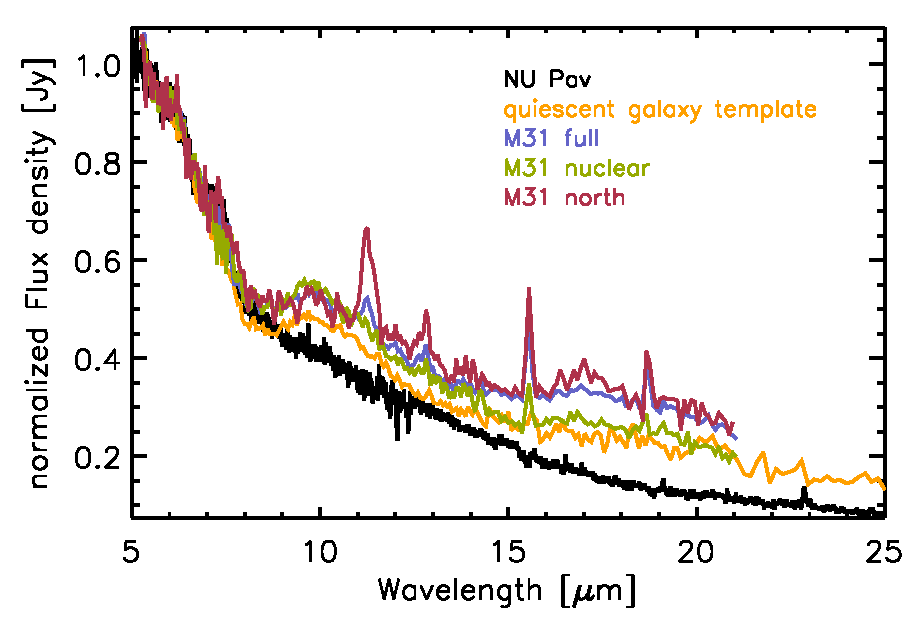
\includegraphics[scale=0.27]{./fig12.eps}
\caption{ PAH equivalent widths versus metallicity. 
Filled circles are M31 7.7~$\mu$m EQWs; filled squares are M31 11.3~$\mu$m EQWs; 
open circles are 7.7~$\mu$m EQWs for the starburst sample from \citet{Engelbracht_2008}.
Metallicities of the M31 regions have had 0.35~dex subtracted to account for the offset  between direct and strong-line measurements. 
}
\label{metalicityVseqw}
\end{figure}

Figure \ref{metalicityVseqw} shows the normalized EQWs of the PAH features  versus the metallicity for our sample and the starburst 
galaxies of \citet{Engelbracht_2008}. The scatter in our sample is large, but the 	
equivalent widths of the 7.7 and 11.3~$\mu$m features are consistent with those of \citet{Engelbracht_2008}. 
No trend with metallicity is seen.
However, we do not have enough data from low-metallicity regions in M31 to observe the expected decrease of EQWs of PAH with the decreasing 
metallicity.  There do seem to be some outliers which can plausibly be due to the uncertainties  and the offset between different methods of calculating the metallicity.  
The M31 region with very low  7.7~$\mu$m  equivalent widths is Region 8, which has
a noisy spectrum in the blue as well as substantial modelled contribution from starlight (see Figure~\ref{PAHFITplots}).



\subsection{Mid-infrared properties of the M31 nucleus}
\label{sect:nucleus}


Examining the {\em Spitzer}-IRS spectral data cube for the nuclear region, we noticed that different spectral features vary spatially in the near-nuclear region.
The 11.2~$\mu$m PAH emission is discrete and patchy (Figure \ref{nuc11} (top)).  Indeed, the majority of the 11.2~$\mu$m  PAH emission is from a region 15\arcsec\ north of the nucleus (
00:42:43.947, +41:16:22.92) and not from the nucleus itself. Weaker 11.2~$\mu$m PAH emission is also found near the edge of the map peaking at (0:42:45.497, +41:15:43.97) and near (0:42:45.869;+41:16:11.38).
On the other hand, the centre shows no PAH emission, but it does have silicate emission around 9.7~$\mu$m, which comes only from the nucleus and is not present in the North region (Figure \ref{nuc11} (middle)).%
\footnote{The spatial resolution and pixel scale of the ISOCAM data are not sufficient to resolve these two regions.}
Finally, the spatial morphology of the [NeIII] 15.5~$\mu$m line emission is present across the nuclear region and thus distinct from that of the silicate and PAH emission (Figure \ref{nuc11} (bottom)). However, the [NeIII] 15.5~$\mu$m line emission is strong at the three locations with 11.2~$\mu$m PAH emission and weak(er) at the nucleus. The locations of the two weaker 11.2~$\mu$m PAH emission peaks are also near positions exhibiting CO(2-1) line emission \citep[\#36 and 28 of][the strongest 11.2~$\mu$m PAH emission peak is outside the CO FOV]{Melchior2013}. 
Radial profiles of both the nuclear and north sources have full widths at half maximum (FWHM) of 5--7\arcsec\ 
depending on the wavelength (corresponding to 19--27pc), while the SL PSF FWHM is 2.5--3\arcsec; therefore both sources are marginally spatially resolved.  
We extracted spectra from the centre and the North regions using  $9\arcsec \times 9\arcsec$ 
square apertures as shown in Figures~\ref{fig:nuc_pahfit}, ~\ref{fig:nuc_silicates} and~\ref{smithspec}. 
Both spectra show a blue continuum and atomic fine-structure lines but they exhibit distinct dust emission consistent with the spatial maps: PAH emission is detected in the north spectrum while silicate emission is seen towards the nucleus. 

\begin{figure}
\centering
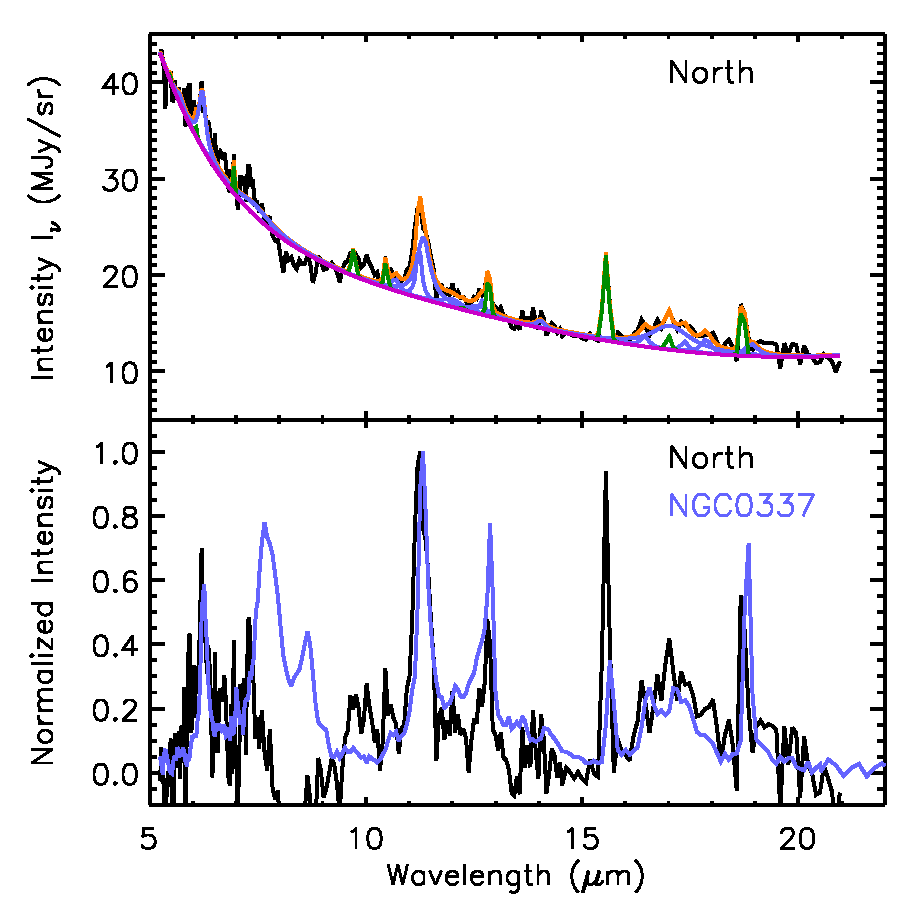
\includegraphics[scale = 0.25]{./fig13a.eps}
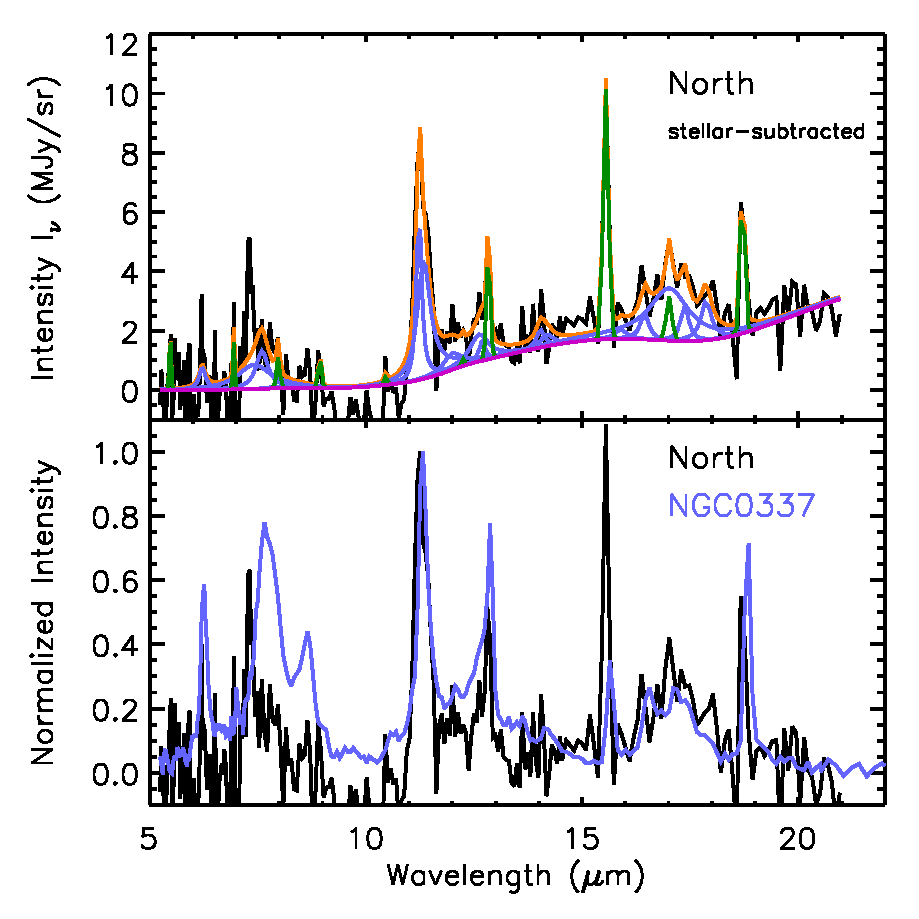
\includegraphics[scale = 0.25]{./fig13b.eps}
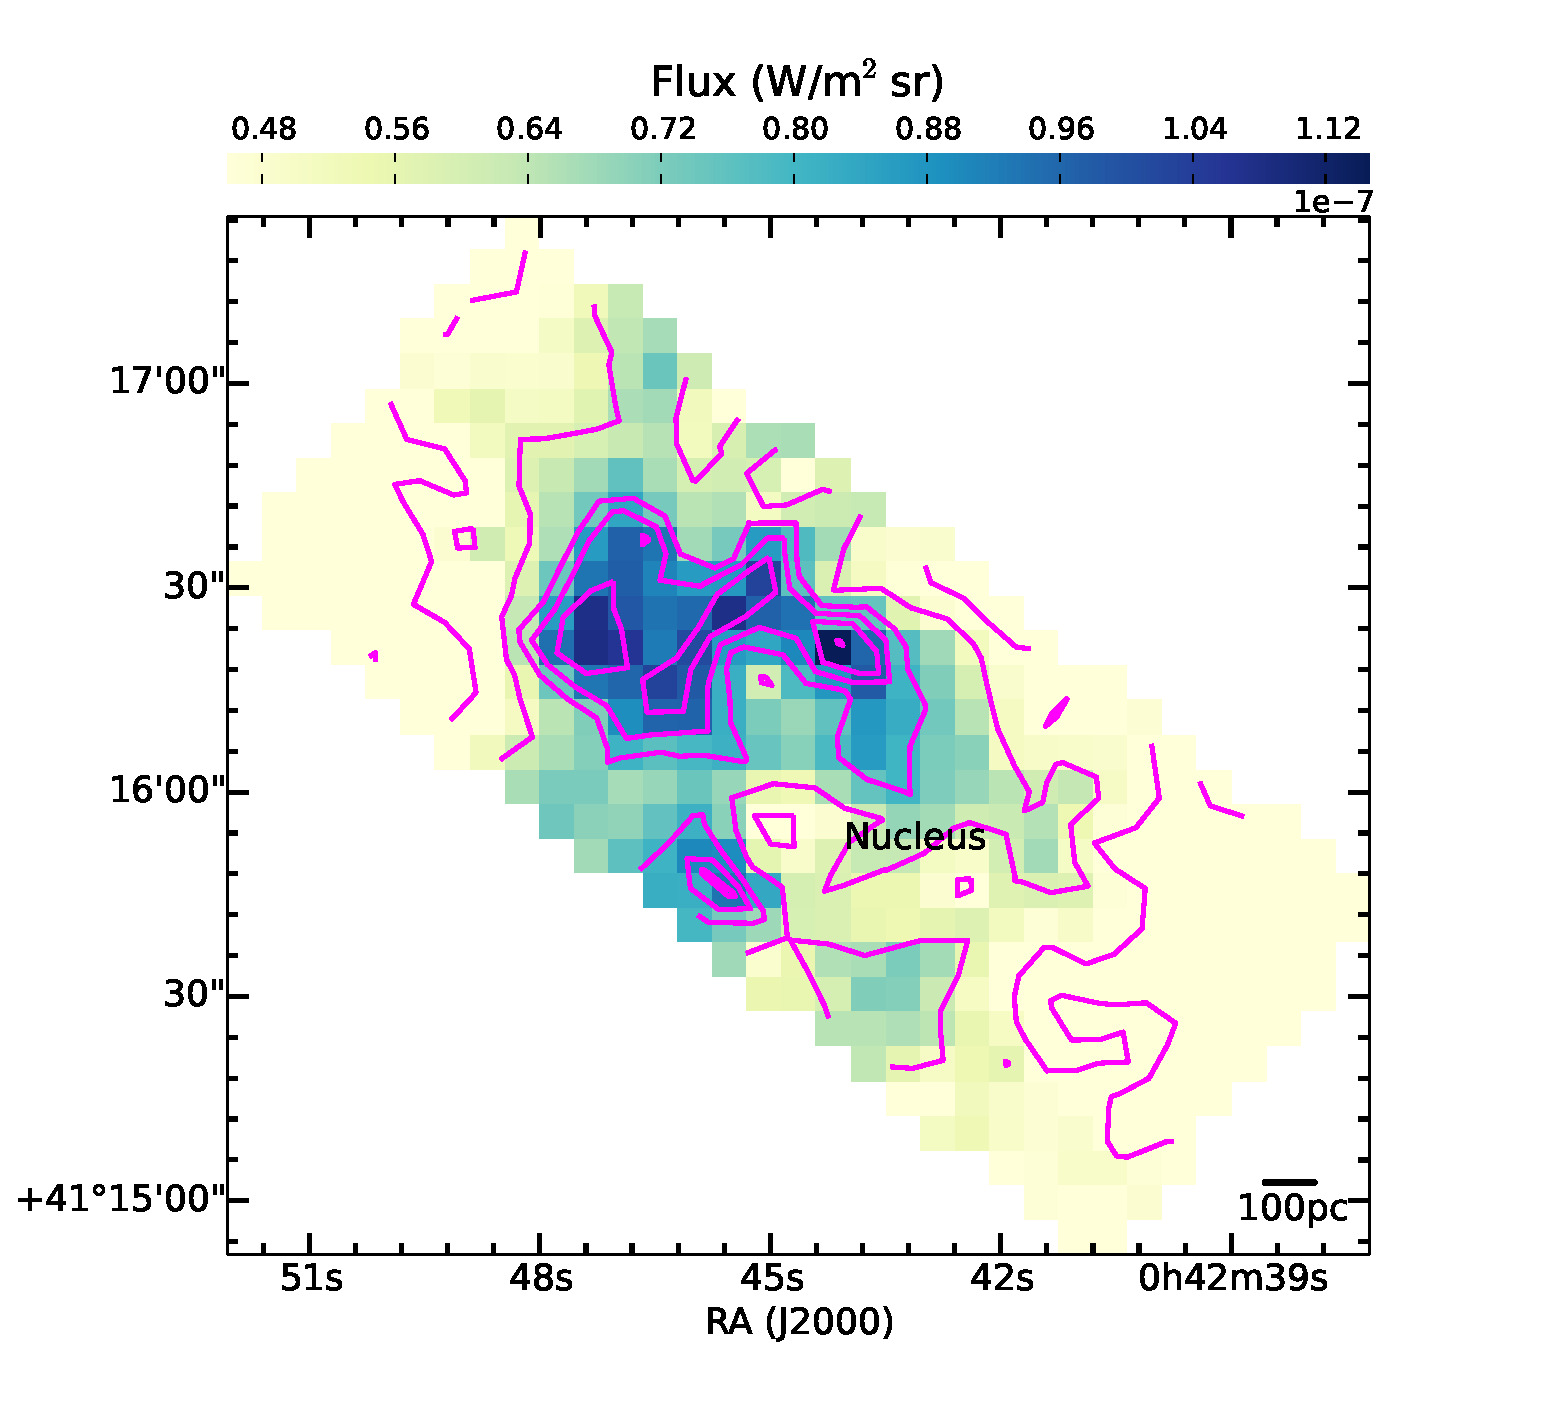
\includegraphics[scale = 0.25]{./fig13c.eps}
\caption{
Integrated strength of the 11.2~$\mu$m PAH emission (top panel), the silicate emission (from 9 to 11~$\mu$m, continuum subtracted; middle panel) and the [NeIII] 15.5~$\mu$m line emission (bottom panel) around the nucleus of M31. As a reference, the [NeIII] 15.5~$\mu$m line emission is shown as contours in each panel. 
The centre of the nucleus is at R.A. $00^{\rm h}42^{\rm m}44\fs35$, Dec. $+41\degr16\arcmin08\farcs5$ \citep{NucleusREF} and is represented by a + sign.  
Two black boxes are the apertures (centre and north region) used to extract spectra.  
{\bf UPDATE BOTTOM PANEL FIGURE WITH NEW FIGURE BY DIMUTHU}
}
\label{nuc11}
\end{figure}


Figure~\ref{fig:nuc_pahfit} (top) shows the results of PAHFIT applied to the spectrum of the north region. Atomic fine-structure lines of Ne and S are detected as well as H$_2$ emission at 17~$\mu$m. In addition, PAH emission is clearly detected at 11.3~$\mu$m and at 15-20~$\mu$m while it is weak or absent at 6--8~$\mu$m. We compared the PAH emission with that of the HII-type galaxy NGC0337 in Figure~\ref{fig:nuc_pahfit} (bottom). Despite the enhanced noise level at the shorter wavelengths, it is clear that the emission shortwards of 10 $\mu$m is atypical for PAHs but rather seem to exhibit a broad plateau from $\sim$6 to $\sim$7.5 $\mu$m. Indeed, 6.2~$\mu$m  PAH emission may be hidden in this broad plateau but the typical 7.7 and 8.6~$\mu$m are absent resulting in a decrease of the 7.7/11.2 ratio by roughly a factor of 10 compared to that of NGC0337. This is consistent with the atypical PAH emission in some low-luminosity active galactic nuclei (LLAGN) reported by \citet{Smith:2007lr}.

The central spectrum exhibit silicate emission, blue continuum emission and fine-structure line emission of [NeII] at 12.8$\mu$m, [NeIII] at 15.5$\mu$m and [SIII] at 18.7$\mu$m (Figure~\ref{fig:nuc_silicates}, top). We adapted PAHFIT so that it includes Gaussian profiles to represent the silicate emission and used this modified PAHFIT to fit the continuum emission of both star light and dust towards the nucleus (Figure~\ref{fig:nuc_silicates}, top). While the silicate emission is not well fitted due to its asymmetry, the underlying continuum is well represented by the PAHFIT results. To characterize the silicate emission profile, we compared the continuum-subtracted silicate profile with the silicate absorption profile of the Galactic centre \citep{Chiar2006} as well as the silicate emission profile observed towards the type 1 (i.e., face-on) LINER nucleus of M81 \citep[][Figure~\ref{fig:nuc_silicates}, bottom]{Smith2010}. For the latter, we adopted a spline continuum anchored at 8.36, 8.83, 24.7, 26.45, and 27.79 $\mu$m (Figure~\ref{fig:nuc_silicates}, middle). Compared to the silicate absorption profile towards the Galactic centre, the M31 silicate emission is clearly displaced towards longer wavelengths and the red wing is slightly less steep resulting in a slightly broader profile. This is consistent with previous results reporting that the silicate emission towards  the M81 nucleus as well as towards several galaxies is redshifted and broader than the silicate absorption seen towards galactic sources \citep[e.g.][]{Sturm2005, Sturm2006, Netzer2007, Smith2010}. Contrasting the spectral properties of the nuclei of M31 and M81, we find that the ``9.7"~$\mu$m silicate emission is distinct from each other in peak position (9.9 and 10.56 $\mu$m respectively) and FWHM (2.58 and 2.79 $\mu$m respectively).\footnote{The reported FWHM is smaller than that reported by \citet{Smith2010} as we consider the continuum-subtracted silicate emission profile.} Moreover, the physical size of the silicate emitting region is much smaller in M31 (19--27pc with respect to 230pc for M81). And while M31 has no PAH emission in its nuclear centre, PAH emission is present across the nuclear region in M81. However, it is atypical in the same way as the PAH emission seen 15" North of M31's nuclear centre. Finally, also the atomic lines (e.g. [Ne {\sc ii}]~12.8~$\mu$m) are distinct between both nuclei. 

\begin{figure}
\centering
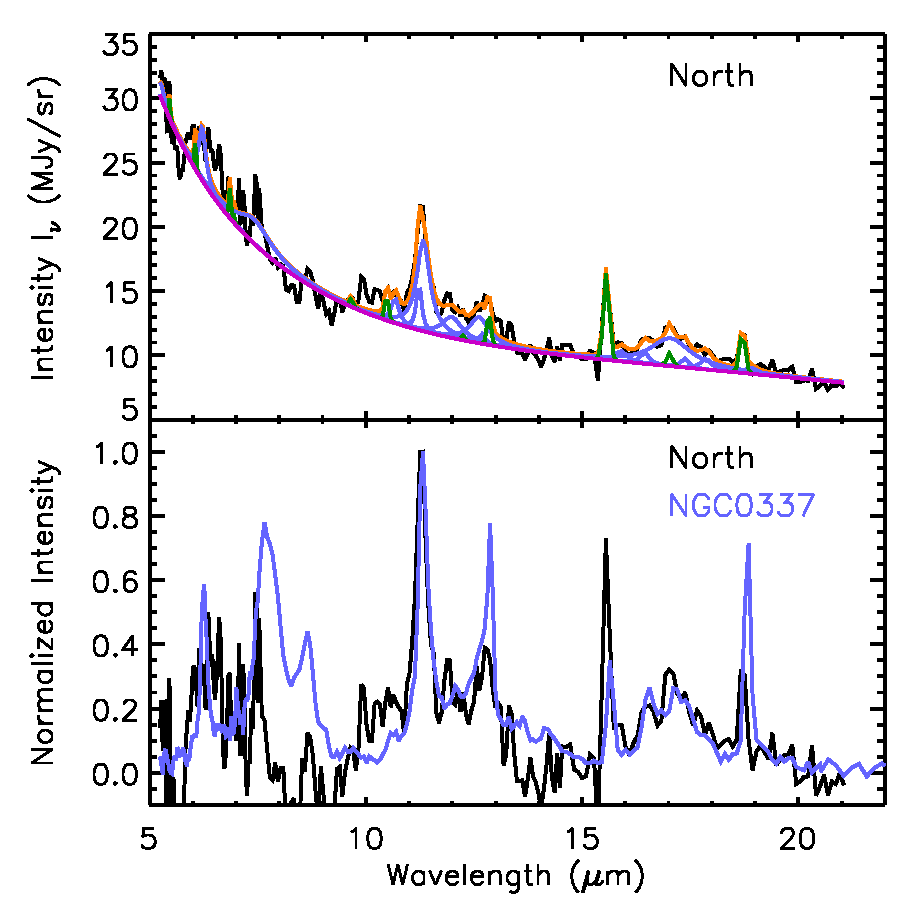
\includegraphics[width = 8 cm]{./fig14.eps}
\caption{Top: PAHFIT result for the extracted spectrum from the north region of the M31 nucleus: fit (orange), continuum (magenta), individual dust components (blue), individual fine-structure lines and H$_2$ lines (green). Bottom: Continuum subtracted spectrum of the north region compared with that of the HII-type galaxy NGC0337 \citep{Smith:2007lr}, normalized to the peak intensity of the  11.2~$\mu$m PAH emission. PAH emission is clearly present longward of~10 $\mu$m. }
\label{fig:nuc_pahfit}
\end{figure}

\begin{figure}
\centering
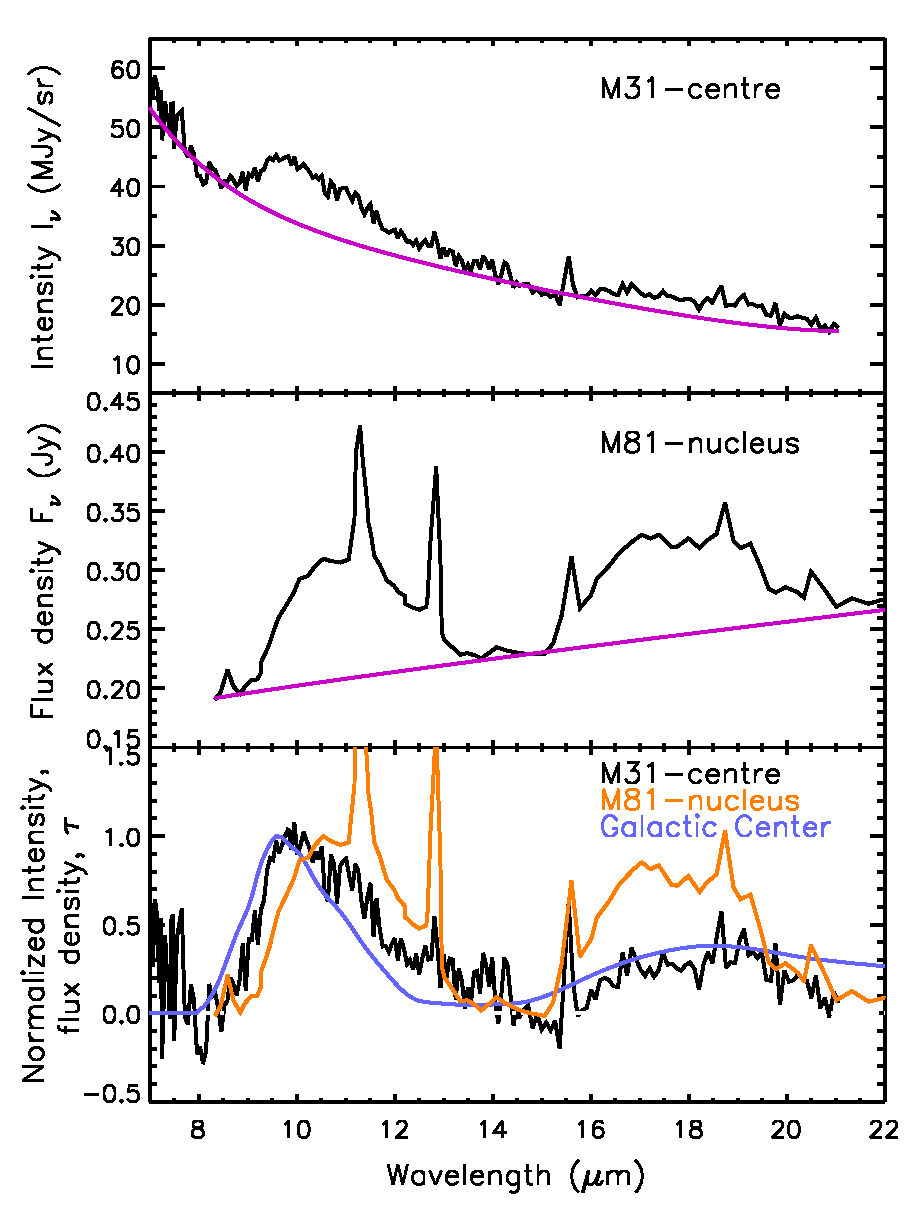
\includegraphics[width = 8 cm]{./fig15.eps}
\caption{Top: Mid-infrared spectrum from the centre region of the M31 nucleus (black) with continuum (magenta). Middle:  Mid-infrared spectrum of the nucleus of M81 \citep[13\arcsec$\times$13\arcsec aperture][black]{Smith2010} with continuum (magenta). Bottom: Normalized continuum-subtracted spectra of the M31 and M81 nuclei. For reference, the silicate optical depth profile towards the galactic centre is shown in blue \citep{Chiar2006}.}
\label{fig:nuc_silicates}
\end{figure}


\begin{figure*}
\centering
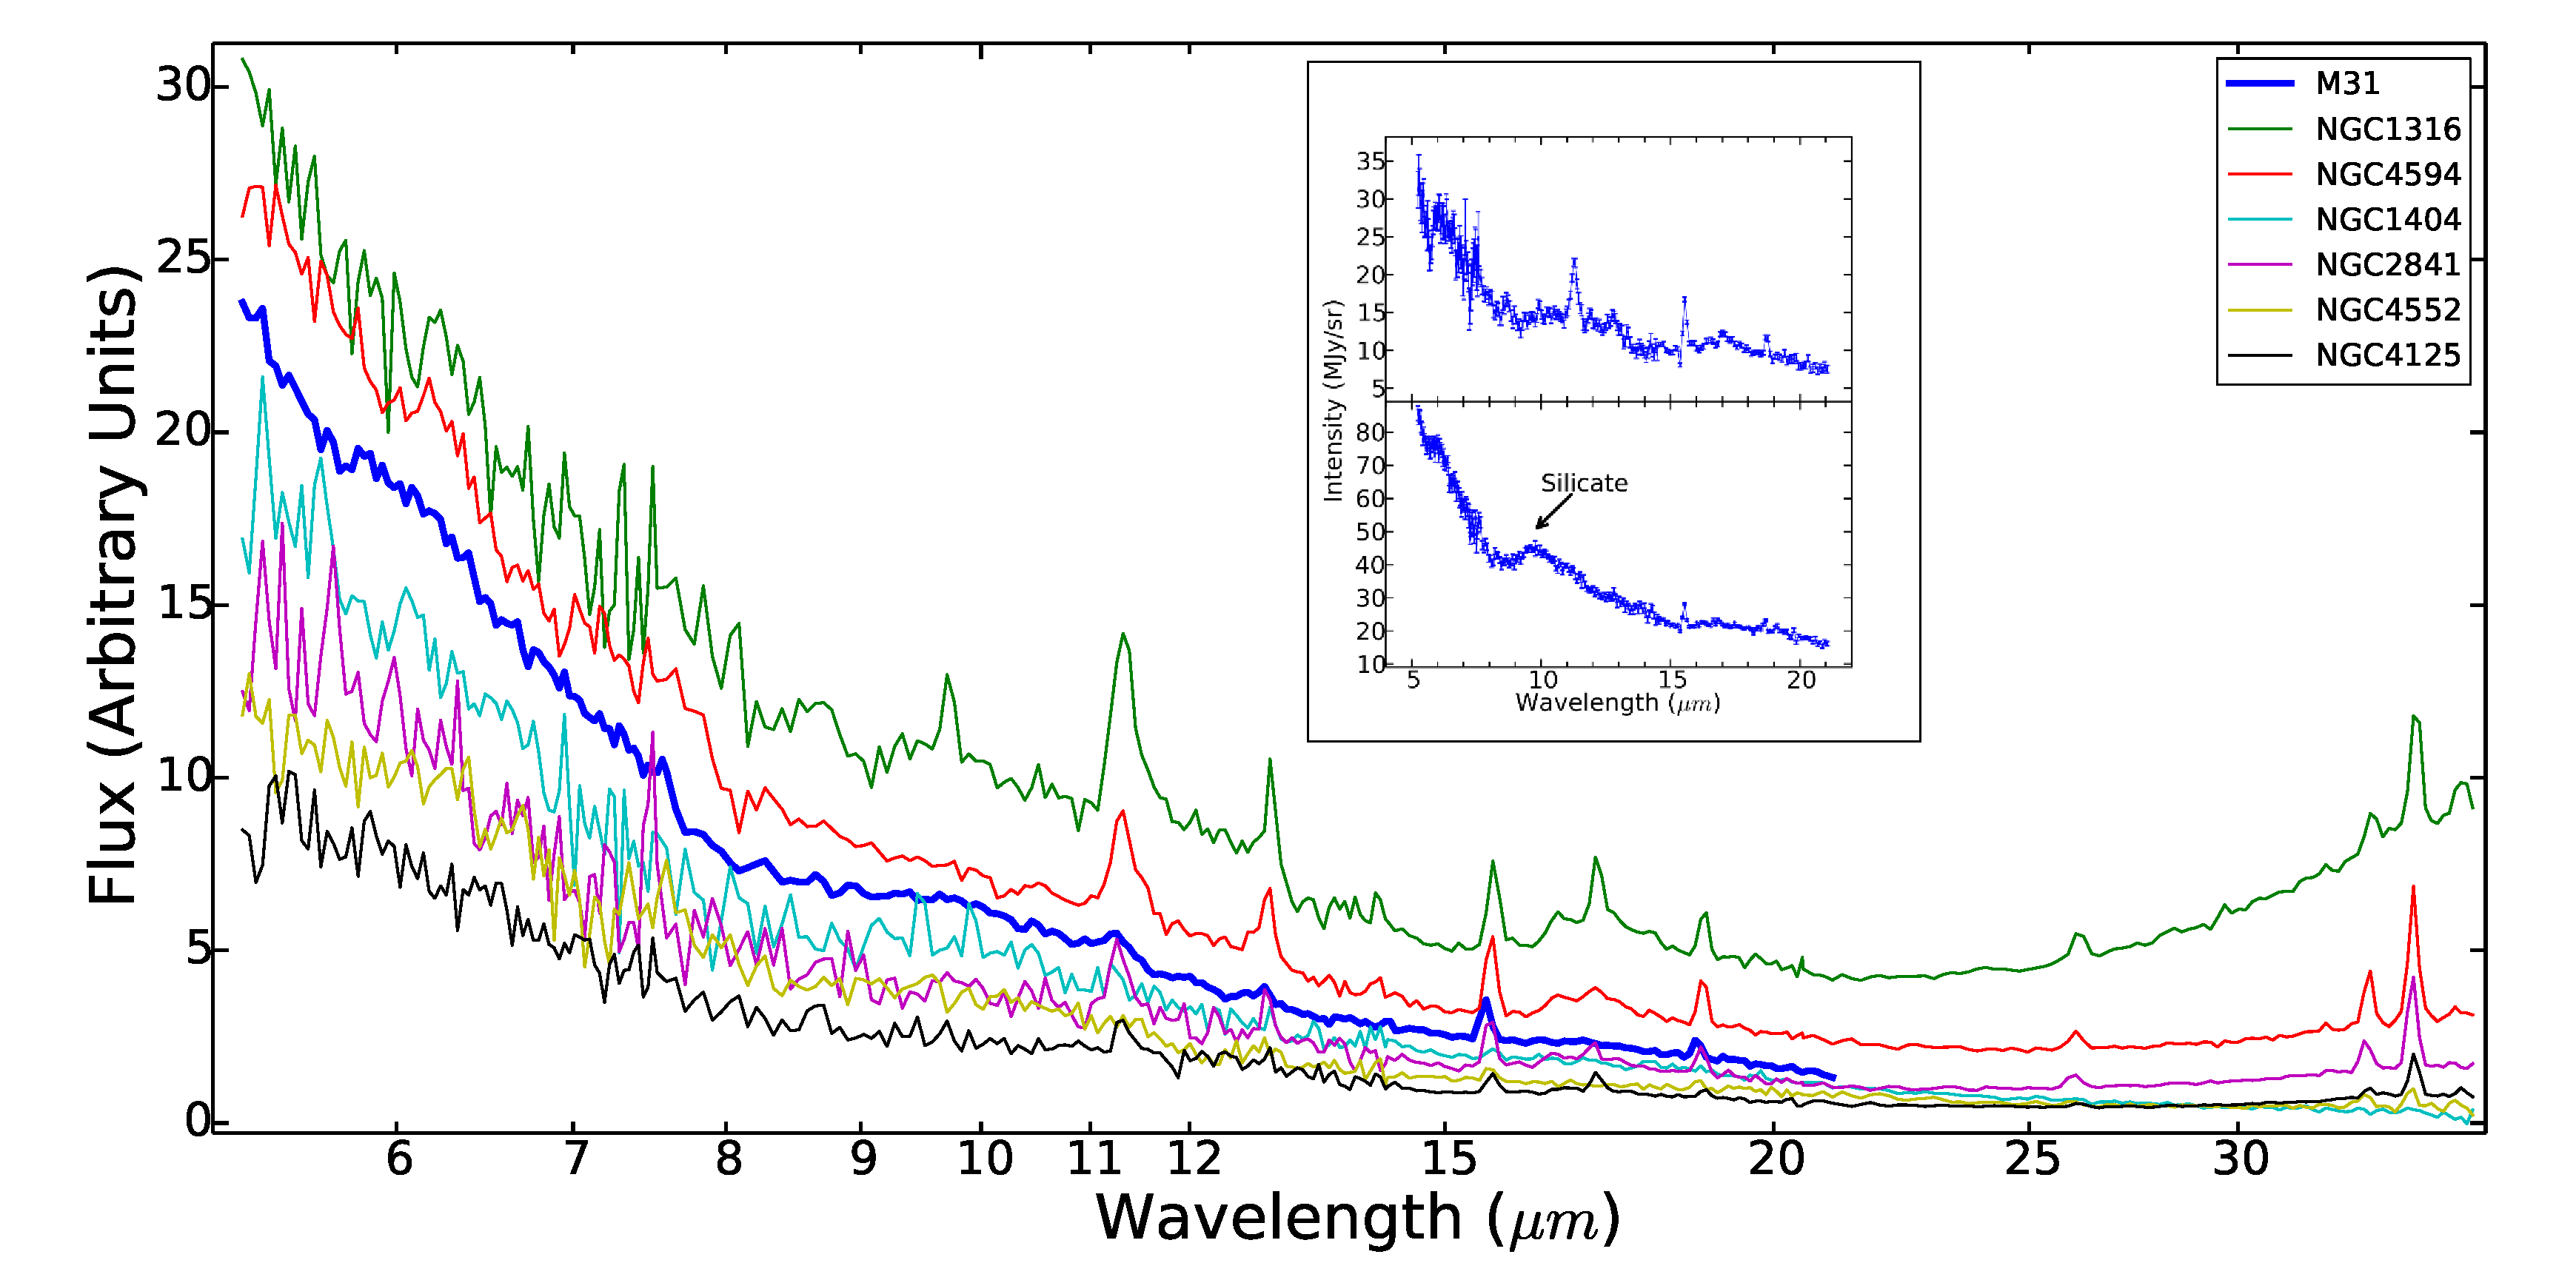
\includegraphics[height = 8 cm]{./fig16.eps}
\caption{Mid-infrared spectrum of the nucleus of M31 (blue) over-plotted with spectra extracted close to the nuclei of 6 nearby galaxies which have 
AGN activity \citep{Smith:2007lr}. NGC 4552, NGC 1404 and NGC 4125 are elliptical galaxies and NGC 4594 and NGC 2841 are spiral galaxies. 
NGC 1316 is a lenticular galaxy. The inset shows the spectra extracted from the centre region of the M31 nucleus (bottom) and from the north region (top) 
shown in Figure \ref{nuc11}.}
\label{smithspec}
\end{figure*}

Figure \ref{smithspec} compares the full 30\arcsec $\times$ 50\arcsec\ M31 nuclear spectrum with the spectra extracted from the smaller regions in the centre and the North (inset, top and bottom). Also shown are nuclear spectra
from six SINGS galaxies with similar spectral shapes \citep{Smith:2007lr}.% 
\footnote{The IRS spectra for the SINGS galaxies were extracted over areas ranging from 2 to 8 kpc$^2$, whereas the M31
nucleus spectrum covers a much smaller area (0.02~kpc$^2$).}
Some SINGS galaxies share similar PAH feature characteristics to the M31 spectrum and none of them contains obvious silicate emission. Although \citet{Mason2012} reported silicate emission towards NGC4594. 
All of these comparison galaxies have some type of LLAGN.
The SINGS galaxies with similar spectral shapes include  three elliptical galaxies, two spirals, and a lenticular; there is some disagreement over the
exact nuclear spectral types of these six galaxies \citep{kennicutt03,Smith:2007lr, moustakas2010}.  All are classified as some form of LLAGN
such as Seyfert or LINER \citep[luminous AGNs were intentionally omitted from the SINGS sample;][]{kennicutt03}, although they are
by no means the only LLAGNs in the SINGS sample.
Published estimates of the black hole masses for these galaxies range from $1.5-5.5\times10^{8}$~M$_{\sun}$
\citep[for NGC~1316 and NGC~4595, respectively]{nowak08, kormendy88}, or about $1-4\times$ that of M31.
M81 is classified as a LINER, with a black hole mass of $7\times10^7$~M$_{\sun}$ \citep{devereux03}.
\citet{Li09} concluded that the central black hole in M31 (M31*) is currently inactive, with direct observational signatures seen only
at radio and X--ray wavelengths, so finding additional signatures in the mid-infrared is of great interest.
To our knowledge, no such signatures have been reported; broadband mid-infrared imaging of the central 
regions of M31 \citep{davidge06,Barmby2006lr} did not identify unambiguous nuclear emission. The bluest
part of the spectrum in Figure~\ref{smithspec} is dominated by the continuum, in agreement with the
expectation that stellar light dominates the nucleus at these wavelengths.


Could radiation from M31* be responsible for the suppression of the  6--8~$\mu$m PAH features compared
to the 11.3~$\mu$m feature?
As discussed by  \citet{Smith:2007lr} and \citet{Smith2010}, inferring such a suppression must be done with caution, 
because the 6--8~$\mu$m features are more susceptible to dilution by the stellar continuum. 
Several connections between PAH suppression and the presence of an AGN are possible, including destruction of small PAH molecules by a hard radiation field, modification of the structure of the PAH molecules, or weak ultraviolet continuum from low star formation rates 
leading to decreased PAH excitation \citep{Smith:2007lr, Diamond2010}.  In the latter case, the AGN is not the cause of the suppressed  6--8~$\mu$m features but rather is only detectable when the nuclear star formation rate is low.
Previous work has found low rates of star formation in the centre of M31: although \citet{Melchior2013} found a significant 
amount of cold gas in the centre of the galaxy, this gas does not appear to be associated with current star formation \citep[see also][]{Li09}.
In modelling the far-infrared spectral energy distribution, \cite{Groves2012} found that  
the old stellar population in the M31 bulge is sufficient to heat the observed dust; no young stellar population is needed. We conclude that PAH feature ratios cannot provide direct evidence for radiation from M31*.


Detection of silicate emission in the M31 nuclear spectrum is another possible indicator of nuclear accretion.
Silicate emission is not very common in integrated spectra of galaxies \citep{Spoon2007} but is seen in luminous 
quasar spectra \citep[e.g.][]{Hill14} and, as mentioned above, in the spectrum of the M81 nucleus. 
In the unified model of AGNs, an obscuring torus viewed face-on would be expected to show silicate emission
\citep{AGNtypes1995, AGNref}; however such a view would also be expected to show forbidden atomic lines such as [Ne~{\sc v}] and [S~{\sc iv}],
not seen in the M31 spectrum. Alternatively, \citet{Mason2012} explained that low-luminosity AGNs cannot 
host a Seyfert-like obscuring torus because of their optically thin dust and low dust-to-gas ratio, but can show
silicate emission that originates in the optically thin hot dust around the central engine.  The first detection of such silicate emission was 
reported by \citet{Sturm2005} from the low-ionization nuclear emission-line region (LINER) galaxy NGC~3998, and 
\citet{Mason2012}  observed that  9.7~$\mu$m silicate emission is present in many LLAGNs. 
To quantify the magnitude of the silicate emission in mid-infrared spectra, \citet{Smith2010} defined
the linear slope parameter $\gamma810 =[F_{\nu}(10\mu{\rm m}) -F_{\nu}(8\mu{\rm m})]/2F_{\nu}(9\mu{\rm m})$,
with positive values signifying silicate emission and negative values absorption. They found the M81 nucleus to have
$\gamma810=0.37\pm0.04$. For the M31 centre (9\arcsec $\times$ 9\arcsec) spectrum, we computed  $\gamma810 =0.01\pm 0.03$,
indicative of neither absorption nor emission. However, for the continuum-subtracted spectrum, we measured   $\gamma810 =1.6\pm 0.4$. This combined with the similar characteristics of the silicate profile in M31 and M81, gives a much stronger indication that silicate emission is detected from M31*.

Measuring the radiated power from the M31 central engine can constrain the geometry and history of the emitting region. 
As discussed by \citet{spinoglio95}, for both active and normal galaxies, the 12~$\mu$m luminosity 
is about 7\% of the bolometric luminosity. With the important caveat that we are discussing only the nucleus,
and not the entire galaxy, we  can use the infrared spectrum to estimate the bolometric luminosity  of the M31 nucleus.
For the centre spectrum, we measure a 12~$\mu$m flux density of 
$0.062 \pm 0.002$~Jy, which corresponds to a 12~$\mu$m luminosity of $(1.13\pm0.03) \times10^{39}$ erg~s$^{-1}$ and a bolometric luminosity
of  $(1.62\pm0.01) \times10^{40}$ erg~s$^{-1}$ ($\log L_{\rm bol} = 40.21$). 
This value is well within the range defined for low-luminosity AGN \citep[$\log L_{\rm bol} <42$,][]{Mason2012}, and
implies an Eddington ratio $L_{\rm bol}/L_{\rm Edd} \sim 10^{-7}$ for a black hole mass of $10^8$~M$_{\sun}$. 
Although the bolometric luminosity estimated from the mid-infrared is a factor of $10^3$ times the bolometric
luminosity estimated from the X--ray flux by \citet{Li09}, it certainly agrees with the general conclusion that the M31 nucleus radiates extremely inefficiently.
A high infrared-to-X--ray ratio could indicate that the nucleus was brighter in the recent past and is now cooling;
detailed modeling of the nucleus would require better constraints on the spectral energy distribution and is hence beyond the scope of this work.



\section{Summary and conclusions}
\label{sect:summary}

We  obtained {\em Spitzer}/IRS spectral maps of 12 regions within M31 covering wavelengths 5--21~$\mu$m. 
The spectra from those regions, except for the nucleus, are similar to spectra obtained from other nearby  star-forming galaxies. 
Early  ISOCAM observations towards 4 regions of M31 showing a suppression 
of the 6--8~$\mu$m features' strength and an enhancement of  the 11.3~$\mu$m feature intensity and FWHM \citep{1998Cesarsky} were likely affected by the background subtraction methods applied.

We recover the well-known strong correlation between the 6.2/11.2 and 7.7/11.2 $\mu$m PAH intensity ratios that is governed by the PAH charge balance.  This is another indicator that the PAH emission in all regions but the nucleus is typical. The PAH EQWs in M31 regions show a decreasing trend with increasing radiation hardness, consistent with previous 
results from other nearby galaxies. The distribution of PAH EQWs with metallicity is well within the range of the starburst galaxy sample of \citet{Engelbracht_2008}. 
We did not have enough data from low-metallicity regions of M31 to observe the decreasing trend of EQWs at low metallicities which is visible in other galaxies.

Different spectral features (11.2~$\mu$m PAH emission, [NeIII] 15.5~$\mu$m line emission, silicate emission) show distinct spatial distributions in the nuclear region. Mid-infrared spectra from near the nucleus of M31 show either suppressed 6--8~$\mu$m features and a strong 11.3~$\mu$m feature
(15\arcsec off-nucleus) or silicate emission around 9.7~$\mu$m  (on-nucleus). The silicate emission profile is redshifted and broader than that observed towards the Galactic centre, in line with previous results from other galaxies and the M81 nucleus.  We contrast the spectral properties of the nuclei of M31 and M81 and find differences in the peak position and FWHM of the silicate feature, the silicate emitting region, the PAH emission, and the fine-structure line emission. 
The nuclear spectrum is similar to that of six other nearby galaxies known to have low luminosity AGN activity. This could strengthen the
suggestion by \citet{Smith:2007lr} that low $L(7.7\mu{\rm m})/L(11.3\mu{\rm m})$ is an indicator of low luminosity AGN. 
The nuclear silicate emission is another possible AGN indicator.
The 12~$\mu$m luminosity can be used to estimate a bolometric luminosity for the M31 nucleus of $1.6\times 10^{40}$~erg~s$^{-1}$,
well within the `low-luminosity' classification, but well above the value estimated from the X--ray flux.


\section*{Acknowledgements}

The authors thank D. Stock, K. Sandstrom and S. Lianou for fruitful discussions and technical support
and S. Gallagher for helpful comments.
We acknowledge support from NSERC Discovery Grants to PB and EP, an NSERC Discovery Accelerator Grant to EP,
and JPL RSAs \# 1369565 and 1279141 to HS.
This work is based on observations made with the {\em Spitzer} Space Telescope, which is operated by the 
Jet Propulsion Laboratory, California Institute of Technology under a contract with NASA.
This research has made use of NASA's Astrophysics Data System.
The version of the ISO data presented in this paper correspond to the Highly Processed Data Product (HPDP) set called `Mid-IR Spectro Imaging ISOCAM CVF Observations'
by \citet{Boulanger_F_2005}, available for public use in the ISO Data Archive.


\bibliographystyle{mn2e}
\begin{thebibliography}{}
\makeatletter
\relax
\def\mn@urlcharsother{\let\do\@makeother \do\$\do\&\do\#\do\^\do\_\do\%\do\~}
\def\mn@doi{\begingroup\mn@urlcharsother \@ifnextchar[{\mn@doi@}{\mn@doi@[]}}
\def\mn@doi@[#1]#2{\def\@tempa{#1}\ifx\@tempa\@empty
  \href{http://dx.doi.org/#2}{doi:#2}\else \href{http://dx.doi.org/#2}{#1}\fi
  \endgroup}
\def\mn@eprint#1#2{\mn@eprint@#1:#2::\@nil}
\def\mn@eprint@arXiv#1{\href{http://arxiv.org/abs/#1}{{\tt arXiv:#1}}}
\def\mn@eprint@dblp#1{\href{http://dblp.uni-trier.de/rec/bibtex/#1.xml}{dblp:#1}}
\def\mn@eprint@#1:#2:#3:#4\@nil{\def\@tempa {#1}\def\@tempb {#2}\def\@tempc
  {#3}\ifx \@tempc \@empty \let\@tempc\@tempb \let\@tempb\@tempa \fi \ifx
  \@tempb \@empty \def\@tempb{arXiv}\fi \@ifundefined
  {mn@eprint@\@tempb}{\@tempb:\@tempc}{\expandafter \expandafter \csname
  mn@eprint@\@tempb\endcsname \expandafter{\@tempc}}}

\bibitem[\protect\citeauthoryear{{Allamandola}, {Tielens}  \&
  {Barker}}{{Allamandola} et~al.}{1989}]{Allamandola1989}
{Allamandola} L.~J.,  {Tielens} A.~G.~G.~M.,   {Barker} J.~R.,  1989, \mn@doi
  [\apjs] {10.1086/191396}, \href
  {http://adsabs.harvard.edu/abs/1989ApJS...71..733A} {71, 733}

\bibitem[\protect\citeauthoryear{{Bacon}, {Emsellem}, {Combes}, {Copin},
  {Monnet}  \& {Martin}}{{Bacon} et~al.}{2001}]{Bacon2001}
{Bacon} R.,  {Emsellem} E.,  {Combes} F.,  {Copin} Y.,  {Monnet} G.,   {Martin}
  P.,  2001, \mn@doi [\aap] {10.1051/0004-6361:20010317}, \href
  {http://adsabs.harvard.edu/abs/2001A%26A...371..409B} {371, 409}

\bibitem[\protect\citeauthoryear{{Barmby} et~al.,}{{Barmby}
  et~al.}{2006}]{Barmby2006lr}
{Barmby} P.,  et~al., 2006, \mn@doi [\apjl] {10.1086/508626}, \href
  {http://adsabs.harvard.edu/abs/2006ApJ...650L..45B} {650, L45}

\bibitem[\protect\citeauthoryear{{Beir{\~a}o}, {Brandl}, {Devost}, {Smith},
  {Hao}  \& {Houck}}{{Beir{\~a}o} et~al.}{2006}]{Beirao:06}
{Beir{\~a}o} P.,  {Brandl} B.~R.,  {Devost} D.,  {Smith} J.~D.,  {Hao} L.,
  {Houck} J.~R.,  2006, \mn@doi [\apjl] {10.1086/505027}, \href
  {http://adsabs.harvard.edu/abs/2006ApJ...643L...1B} {643, L1}

\bibitem[\protect\citeauthoryear{{Bender} et~al.,}{{Bender}
  et~al.}{2005}]{Bender2005}
{Bender} R.,  et~al., 2005, \mn@doi [\apj] {10.1086/432434}, \href
  {http://adsabs.harvard.edu/abs/2005ApJ...631..280B} {631, 280}

\bibitem[\protect\citeauthoryear{{Boulanger} et~al.,}{{Boulanger}
  et~al.}{2005}]{Boulanger_F_2005}
{Boulanger} F.,  et~al., 2005, \mn@doi [\aap] {10.1051/0004-6361:20047119},
  \href {http://adsabs.harvard.edu/abs/2005A%26A...436.1151B} {436, 1151}

\bibitem[\protect\citeauthoryear{{Brandl} et~al.,}{{Brandl}
  et~al.}{2006}]{Brandl2006}
{Brandl} B.~R.,  et~al., 2006, \mn@doi [\apj] {10.1086/508849}, \href
  {http://adsabs.harvard.edu/abs/2006ApJ...653.1129B} {653, 1129}

\bibitem[\protect\citeauthoryear{{Calzetti} et~al.,}{{Calzetti}
  et~al.}{2010}]{Calzetti:2010fk}
{Calzetti} D.,  et~al., 2010, Conference Proceedings `Reionization to
  Exoplanets', ed. P. Ogle, ASP Conference Series, \href
  {http://adsabs.harvard.edu/abs/2010arXiv1005.4644C} {}

\bibitem[\protect\citeauthoryear{{Cesarsky} et~al.,}{{Cesarsky}
  et~al.}{1996}]{cesarsky1996}
{Cesarsky} C.~J.,  et~al., 1996, \aap, \href
  {http://adsabs.harvard.edu/abs/1996A%26A...315L..32C} {315, L32}

\bibitem[\protect\citeauthoryear{{Cesarsky}, {Lequeux}, {Pagani}, {Ryter},
  {Loinard}  \& {Sauvage}}{{Cesarsky} et~al.}{1998}]{1998Cesarsky}
{Cesarsky} D.,  {Lequeux} J.,  {Pagani} L.,  {Ryter} C.,  {Loinard} L.,
  {Sauvage} M.,  1998, \aap, \href
  {http://adsabs.harvard.edu/abs/1998A%26A...337L..35C} {337, L35}

\bibitem[\protect\citeauthoryear{{Chiar} \& {Tielens}}{{Chiar} \&
  {Tielens}}{2006}]{Chiar2006}
{Chiar} J.~E.,  {Tielens} A.~G.~G.~M.,  2006, \mn@doi [\apj] {10.1086/498406},
  \href {http://adsabs.harvard.edu/abs/2006ApJ...637..774C} {637, 774}

\bibitem[\protect\citeauthoryear{{Croley}, {Barmby}, {Stock}, {Azimlu}  \&
  {Rosolowsky}}{{Croley} et~al.}{2014}]{Mitchel2014}
{Croley} M.,  {Barmby} P.,  {Stock} D.,  {Azimlu} M.,   {Rosolowsky} E.,  2014,
  MNRAS, submitted

\bibitem[\protect\citeauthoryear{{Davidge}, {Jensen}  \& {Olsen}}{{Davidge}
  et~al.}{2006}]{davidge06}
{Davidge} T.~J.,  {Jensen} J.~B.,   {Olsen} K.~A.~G.,  2006, \mn@doi [\aj]
  {10.1086/505463}, \href {http://adsabs.harvard.edu/abs/2006AJ....132..521D}
  {132, 521}

\bibitem[\protect\citeauthoryear{{Devereux}, {Ford}, {Tsvetanov}  \&
  {Jacoby}}{{Devereux} et~al.}{2003}]{devereux03}
{Devereux} N.,  {Ford} H.,  {Tsvetanov} Z.,   {Jacoby} G.,  2003, \mn@doi [\aj]
  {10.1086/367595}, \href {http://cdsads.u-strasbg.fr/abs/2003AJ....125.1226D}
  {125, 1226}

\bibitem[\protect\citeauthoryear{{Diamond-Stanic} \& {Rieke}}{{Diamond-Stanic}
  \& {Rieke}}{2010}]{Diamond2010}
{Diamond-Stanic} A.~M.,  {Rieke} G.~H.,  2010, \mn@doi [\apj]
  {10.1088/0004-637X/724/1/140}, \href
  {http://adsabs.harvard.edu/abs/2010ApJ...724..140D} {724, 140}

\bibitem[\protect\citeauthoryear{{Efstathiou} \& {Rowan-Robinson}}{{Efstathiou}
  \& {Rowan-Robinson}}{1995}]{AGNtypes1995}
{Efstathiou} A.,  {Rowan-Robinson} M.,  1995, \mnras, \href
  {http://adsabs.harvard.edu/abs/1995MNRAS.273..649E} {273, 649}

\bibitem[\protect\citeauthoryear{{Engelbracht}, {Rieke}, {Gordon}, {Smith},
  {Werner}, {Moustakas}, {Willmer}  \& {Vanzi}}{{Engelbracht}
  et~al.}{2008}]{Engelbracht_2008}
{Engelbracht} C.~W.,  {Rieke} G.~H.,  {Gordon} K.~D.,  {Smith} J.-D.~T.,
  {Werner} M.~W.,  {Moustakas} J.,  {Willmer} C.~N.~A.,   {Vanzi} L.,  2008,
  \mn@doi [\apj] {10.1086/529513}, \href
  {http://adsabs.harvard.edu/abs/2008ApJ...678..804E} {678, 804}

\bibitem[\protect\citeauthoryear{{Galliano}, {Madden}, {Tielens}, {Peeters}  \&
  {Jones}}{{Galliano} et~al.}{2008a}]{Galliano:08}
{Galliano} F.,  {Madden} S.,  {Tielens} A.,  {Peeters} E.,   {Jones} A.,
  2008a, \apj, 679, 310

\bibitem[\protect\citeauthoryear{{Galliano}, {Madden}, {Tielens}, {Peeters}  \&
  {Jones}}{{Galliano} et~al.}{2008b}]{Galliano2008}
{Galliano} F.,  {Madden} S.~C.,  {Tielens} A.~G.~G.~M.,  {Peeters} E.,
  {Jones} A.~P.,  2008b, \mn@doi [\apj] {10.1086/587051}, \href
  {http://adsabs.harvard.edu/abs/2008ApJ...679..310G} {679, 310}

\bibitem[\protect\citeauthoryear{{Garcia} et~al.,}{{Garcia}
  et~al.}{2010}]{NucleusREF}
{Garcia} M.~R.,  et~al., 2010, \mn@doi [\apj] {10.1088/0004-637X/710/1/755},
  \href {http://adsabs.harvard.edu/abs/2010ApJ...710..755G} {710, 755}

\bibitem[\protect\citeauthoryear{{Geballe}, {Lacy}, {Persson}, {McGregor}  \&
  {Soifer}}{{Geballe} et~al.}{1985}]{Geballe:85}
{Geballe} T.~R.,  {Lacy} J.~H.,  {Persson} S.~E.,  {McGregor} P.~J.,   {Soifer}
  B.~T.,  1985, \apj, 292, 500

\bibitem[\protect\citeauthoryear{{Gillett}, {Forrest}  \& {Merrill}}{{Gillett}
  et~al.}{1973}]{Gillett:73}
{Gillett} F.~C.,  {Forrest} W.~J.,   {Merrill} K.~M.,  1973, \apj, 183, 87

\bibitem[\protect\citeauthoryear{{Gordon} et~al.,}{{Gordon}
  et~al.}{2006}]{gordon06a}
{Gordon} K.~D.,  et~al., 2006, \mn@doi [\apjl] {10.1086/501046}, \href
  {http://adsabs.harvard.edu/abs/2006ApJ...638L..87G} {638, L87}

\bibitem[\protect\citeauthoryear{{Gordon}, {Engelbracht}, {Rieke}, {Misselt},
  {Smith}  \& {Kennicutt}}{{Gordon} et~al.}{2008}]{Gordon:2008lr}
{Gordon} K.~D.,  {Engelbracht} C.~W.,  {Rieke} G.~H.,  {Misselt} K.~A.,
  {Smith} J.-D.~T.,   {Kennicutt} Jr. R.~C.,  2008, \mn@doi [\apj]
  {10.1086/589567}, \href {http://adsabs.harvard.edu/abs/2008ApJ...682..336G}
  {682, 336}

\bibitem[\protect\citeauthoryear{{Groves} et~al.,}{{Groves}
  et~al.}{2012}]{Groves2012}
{Groves} B.,  et~al., 2012, \mn@doi [\mnras]
  {10.1111/j.1365-2966.2012.21696.x}, \href
  {http://adsabs.harvard.edu/abs/2012MNRAS.426..892G} {426, 892}

\bibitem[\protect\citeauthoryear{{Hao} et~al.,}{{Hao} et~al.}{2005}]{Hao2005}
{Hao} L.,  et~al., 2005, \mn@doi [\apjl] {10.1086/431227}, \href
  {http://adsabs.harvard.edu/abs/2005ApJ...625L..75H} {625, L75}

\bibitem[\protect\citeauthoryear{{Hill}, {Gallagher}, {Deo}, {Peeters}  \&
  {Richards}}{{Hill} et~al.}{2014}]{Hill14}
{Hill} A.~R.,  {Gallagher} S.~C.,  {Deo} R.~P.,  {Peeters} E.,   {Richards}
  G.~T.,  2014, \mn@doi [\mnras] {10.1093/mnras/stt2346}, \href
  {http://adsabs.harvard.edu/abs/2014MNRAS.438.2317H} {438, 2317}

\bibitem[\protect\citeauthoryear{{Hony}, {Van Kerckhoven}, {Peeters},
  {Tielens}, {Hudgins}  \& {Allamandola}}{{Hony} et~al.}{2001}]{Hony:oops:01}
{Hony} S.,  {Van Kerckhoven} C.,  {Peeters} E.,  {Tielens} A.~G.~G.~M.,
  {Hudgins} D.~M.,   {Allamandola} L.~J.,  2001, \aap, 370, 1030

\bibitem[\protect\citeauthoryear{{Houck} et~al.,}{{Houck}
  et~al.}{2004}]{IRS2004}
{Houck} J.~R.,  et~al., 2004, \mn@doi [\apjs] {10.1086/423134}, \href
  {http://adsabs.harvard.edu/abs/2004ApJS..154...18H} {154, 18}

\bibitem[\protect\citeauthoryear{{Hudgins} \& {Allamandola}}{{Hudgins} \&
  {Allamandola}}{2004}]{Hudgins:rev:04}
{Hudgins} D.~M.,  {Allamandola} L.~J.,  2004, in {Witt} A.~N.,  {Clayton}
  G.~C.,   {Draine} B.~T.,  eds,  Astronomical Society of the Pacific
  Conference Series Vol. 309, Astrophysics of Dust. p.~665

\bibitem[\protect\citeauthoryear{{Kennicutt} Jr. et~al.,}{{Kennicutt}
  et~al.}{2003}]{kennicutt03}
{Kennicutt} Jr. R.~C.,  et~al., 2003, \mn@doi [\pasp] {10.1086/376941}, \href
  {http://adsabs.harvard.edu/abs/2003PASP..115..928K} {115, 928}

\bibitem[\protect\citeauthoryear{{Kessler} et~al.,}{{Kessler}
  et~al.}{1996}]{Kessler1996}
{Kessler} M.~F.,  et~al., 1996, \aap, \href
  {http://adsabs.harvard.edu/abs/1996A%26A...315L..27K} {315, L27}

\bibitem[\protect\citeauthoryear{{Kormendy}}{{Kormendy}}{1988}]{kormendy88}
{Kormendy} J.,  1988, \mn@doi [\apj] {10.1086/166904}, 335, 40

\bibitem[\protect\citeauthoryear{{Lauer} et~al.,}{{Lauer}
  et~al.}{1993}]{Lauer1993}
{Lauer} T.~R.,  et~al., 1993, \mn@doi [\aj] {10.1086/116737}, \href
  {http://adsabs.harvard.edu/abs/1993AJ....106.1436L} {106, 1436}

\bibitem[\protect\citeauthoryear{{Li}, {Wang}  \& {Wakker}}{{Li}
  et~al.}{2009}]{Li09}
{Li} Z.,  {Wang} Q.~D.,   {Wakker} B.~P.,  2009, \mn@doi [\mnras]
  {10.1111/j.1365-2966.2009.14918.x}, \href
  {http://adsabs.harvard.edu/abs/2009MNRAS.397..148L} {397, 148}

\bibitem[\protect\citeauthoryear{{Li}, {Garcia}, {Forman}, {Jones}, {Kraft},
  {Lal}, {Murray}  \& {Wang}}{{Li} et~al.}{2011}]{Li2011}
{Li} Z.,  {Garcia} M.~R.,  {Forman} W.~R.,  {Jones} C.,  {Kraft} R.~P.,  {Lal}
  D.~V.,  {Murray} S.~S.,   {Wang} Q.~D.,  2011, \mn@doi [\apjl]
  {10.1088/2041-8205/728/1/L10}, \href
  {http://adsabs.harvard.edu/abs/2011ApJ...728L..10L} {728, L10}

\bibitem[\protect\citeauthoryear{{Madden}}{{Madden}}{2000}]{Madden:00}
{Madden} S.~C.,  2000, \mn@doi [\nar] {10.1016/S1387-6473(00)00050-6}, \href
  {http://adsabs.harvard.edu/abs/2000NewAR..44..249M} {44, 249}

\bibitem[\protect\citeauthoryear{{Mason}, {Levenson}, {Shi}, {Packham},
  {Gorjian}, {Cleary}, {Rhee}  \& {Werner}}{{Mason} et~al.}{2009}]{Mason2009}
{Mason} R.~E.,  {Levenson} N.~A.,  {Shi} Y.,  {Packham} C.,  {Gorjian} V.,
  {Cleary} K.,  {Rhee} J.,   {Werner} M.,  2009, \mn@doi [\apjl]
  {10.1088/0004-637X/693/2/L136}, \href
  {http://adsabs.harvard.edu/abs/2009ApJ...693L.136M} {693, L136}

\bibitem[\protect\citeauthoryear{{Mason} et~al.,}{{Mason}
  et~al.}{2012}]{Mason2012}
{Mason} R.~E.,  et~al., 2012, \mn@doi [\aj] {10.1088/0004-6256/144/1/11}, \href
  {http://adsabs.harvard.edu/abs/2012AJ....144...11M} {144, 11}

\bibitem[\protect\citeauthoryear{{McConnachie}, {Irwin}, {Ferguson}, {Ibata},
  {Lewis}  \& {Tanvir}}{{McConnachie} et~al.}{2005}]{Mcc2005}
{McConnachie} A.~W.,  {Irwin} M.~J.,  {Ferguson} A.~M.~N.,  {Ibata} R.~A.,
  {Lewis} G.~F.,   {Tanvir} N.,  2005, \mn@doi [\mnras]
  {10.1111/j.1365-2966.2004.08514.x}, \href
  {http://adsabs.harvard.edu/abs/2005MNRAS.356..979M} {356, 979}

\bibitem[\protect\citeauthoryear{{Melchior} \& {Combes}}{{Melchior} \&
  {Combes}}{2013}]{Melchior2013}
{Melchior} A.-L.,  {Combes} F.,  2013, \mn@doi [\aap]
  {10.1051/0004-6361/201220204}, \href
  {http://adsabs.harvard.edu/abs/2013A%26A...549A..27M} {549, A27}

\bibitem[\protect\citeauthoryear{{Moustakas}, {Kennicutt}, {Tremonti}, {Dale},
  {Smith}  \& {Calzetti}}{{Moustakas} et~al.}{2010}]{moustakas2010}
{Moustakas} J.,  {Kennicutt} Jr. R.~C.,  {Tremonti} C.~A.,  {Dale} D.~A.,
  {Smith} J.-D.~T.,   {Calzetti} D.,  2010, \mn@doi [\apjs]
  {10.1088/0067-0049/190/2/233}, \href
  {http://adsabs.harvard.edu/abs/2010ApJS..190..233M} {190, 233}

\bibitem[\protect\citeauthoryear{{Mu{\~n}oz-Mateos} et~al.,}{{Mu{\~n}oz-Mateos}
  et~al.}{2009}]{Munoz:09}
{Mu{\~n}oz-Mateos} J.~C.,  et~al., 2009, \mn@doi [\apj]
  {10.1088/0004-637X/703/2/1569}, \href
  {http://adsabs.harvard.edu/abs/2009ApJ...703.1569M} {703, 1569}

\bibitem[\protect\citeauthoryear{{Nagao}, {Maiolino}  \& {Marconi}}{{Nagao}
  et~al.}{2006}]{Nagao2006}
{Nagao} T.,  {Maiolino} R.,   {Marconi} A.,  2006, \mn@doi [\aap]
  {10.1051/0004-6361:20065216}, \href
  {http://adsabs.harvard.edu/abs/2006A%26A...459...85N} {459, 85}

\bibitem[\protect\citeauthoryear{{Netzer} et~al.,}{{Netzer}
  et~al.}{2007}]{Netzer2007}
{Netzer} H.,  et~al., 2007, \mn@doi [\apj] {10.1086/520716}, \href
  {http://adsabs.harvard.edu/abs/2007ApJ...666..806N} {666, 806}

\bibitem[\protect\citeauthoryear{{Nowak}, {Saglia}, {Thomas}, {Bender},
  {Davies}  \& {Gebhardt}}{{Nowak} et~al.}{2008}]{nowak08}
{Nowak} N.,  {Saglia} R.~P.,  {Thomas} J.,  {Bender} R.,  {Davies} R.~I.,
  {Gebhardt} K.,  2008, \mn@doi [\mnras] {10.1111/j.1365-2966.2008.13960.x},
  391, 1629

\bibitem[\protect\citeauthoryear{{Pagani}, {Lequeux}, {Cesarsky}, {Milliard},
  {Lionard}  \& {Sauvage}}{{Pagani} et~al.}{1999}]{Pagani_1999}
{Pagani} L.,  {Lequeux} J.,  {Cesarsky} D.,  {Milliard} B.,  {Lionard} L.,
  {Sauvage} M.,  1999, \aap, 351, 447

\bibitem[\protect\citeauthoryear{{Peeters}}{{Peeters}}{2011}]{Peeters:toledo:11}
{Peeters} E.,  2011, in IAU Symposium. pp 149--161, \mn@eprint {arXiv}
  {1111.3680}, \mn@doi{10.1017/S174392131102494X}

\bibitem[\protect\citeauthoryear{{Puget} \& {Leger}}{{Puget} \&
  {Leger}}{1989}]{puget89}
{Puget} J.~L.,  {Leger} A.,  1989, \mn@doi [\araa]
  {10.1146/annurev.aa.27.090189.001113}, \href
  {http://adsabs.harvard.edu/abs/1989ARA%26A..27..161P} {27, 161}

\bibitem[\protect\citeauthoryear{{Roche}, {Aitken}, {Smith}  \& {Ward}}{{Roche}
  et~al.}{1991}]{Roche1991}
{Roche} P.~F.,  {Aitken} D.~K.,  {Smith} C.~H.,   {Ward} M.~J.,  1991, \mnras,
  \href {http://adsabs.harvard.edu/abs/1991MNRAS.248..606R} {248, 606}

\bibitem[\protect\citeauthoryear{{Sanders}, {Caldwell}, {McDowell}  \&
  {Harding}}{{Sanders} et~al.}{2012}]{Sanders_2011}
{Sanders} N.~E.,  {Caldwell} N.,  {McDowell} J.,   {Harding} P.,  2012, \mn@doi
  [\apj] {10.1088/0004-637X/758/2/133}, \href
  {http://adsabs.harvard.edu/abs/2012ApJ...758..133S} {758, 133}

\bibitem[\protect\citeauthoryear{{Sandstrom} et~al.,}{{Sandstrom}
  et~al.}{2012}]{Sandstrom12}
{Sandstrom} K.~M.,  et~al., 2012, \mn@doi [\apj] {10.1088/0004-637X/744/1/20},
  \href {http://adsabs.harvard.edu/abs/2012ApJ...744...20S} {744, 20}

\bibitem[\protect\citeauthoryear{{Skillman}, {Terlevich}  \&
  {Terlevich}}{{Skillman} et~al.}{1998}]{Skillman1998}
{Skillman} E.~D.,  {Terlevich} E.,   {Terlevich} R.,  1998, \ssr, \href
  {http://adsabs.harvard.edu/abs/1998SSRv...84..105S} {84, 105}

\bibitem[\protect\citeauthoryear{{Smith} et~al.,}{{Smith}
  et~al.}{2007a}]{Smith:2007fk}
{Smith} J.-D.~T.,  et~al., 2007a, \mn@doi [\pasp] {10.1086/522634}, \href
  {http://adsabs.harvard.edu/abs/2007PASP..119.1133S} {119, 1133}

\bibitem[\protect\citeauthoryear{{Smith} et~al.,}{{Smith}
  et~al.}{2007b}]{Smith:2007lr}
{Smith} J.-D.~T.,  et~al., 2007b, \mn@doi [\apj] {10.1086/510549}, \href
  {http://adsabs.harvard.edu/abs/2007ApJ...656..770S} {656, 770}

\bibitem[\protect\citeauthoryear{{Smith} et~al.,}{{Smith}
  et~al.}{2010}]{Smith2010}
{Smith} H.~A.,  et~al., 2010, \mn@doi [\apj] {10.1088/0004-637X/716/1/490},
  \href {http://adsabs.harvard.edu/abs/2010ApJ...716..490S} {716, 490}

\bibitem[\protect\citeauthoryear{{Spinoglio} \& {Malkan}}{{Spinoglio} \&
  {Malkan}}{1992}]{AGNref}
{Spinoglio} L.,  {Malkan} M.~A.,  1992, \mn@doi [\apj] {10.1086/171943}, \href
  {http://adsabs.harvard.edu/abs/1992ApJ...399..504S} {399, 504}

\bibitem[\protect\citeauthoryear{{Spinoglio}, {Malkan}, {Rush}, {Carrasco}  \&
  {Recillas-Cruz}}{{Spinoglio} et~al.}{1995}]{spinoglio95}
{Spinoglio} L.,  {Malkan} M.~A.,  {Rush} B.,  {Carrasco} L.,   {Recillas-Cruz}
  E.,  1995, \mn@doi [\apj] {10.1086/176425}, \href
  {http://adsabs.harvard.edu/abs/1995ApJ...453..616S} {453, 616}

\bibitem[\protect\citeauthoryear{{Spitzer Science Center}}{{Spitzer Science
  Center}}{2012}]{SpitzerDAC}
{Spitzer Science Center} 2012, {Spitzer Data Analysis Cookbook}, v5.0.1 edn.
SSC, Pasadena, CA

\bibitem[\protect\citeauthoryear{{Spoon}, {Marshall}, {Houck}, {Elitzur},
  {Hao}, {Armus}, {Brandl}  \& {Charmandaris}}{{Spoon}
  et~al.}{2007}]{Spoon2007}
{Spoon} H.~W.~W.,  {Marshall} J.~A.,  {Houck} J.~R.,  {Elitzur} M.,  {Hao} L.,
  {Armus} L.,  {Brandl} B.~R.,   {Charmandaris} V.,  2007, \mn@doi [\apjl]
  {10.1086/511268}, \href {http://adsabs.harvard.edu/abs/2007ApJ...654L..49S}
  {654, L49}

\bibitem[\protect\citeauthoryear{{Stock}, {Peeters}, {Tielens}, {Otaguro}  \&
  {Bik}}{{Stock} et~al.}{2013}]{Stock:13}
{Stock} D.~J.,  {Peeters} E.,  {Tielens} A.~G.~G.~M.,  {Otaguro} J.~N.,   {Bik}
  A.,  2013, \mn@doi [\apj] {10.1088/0004-637X/771/1/72}, \href
  {http://adsabs.harvard.edu/abs/2013ApJ...771...72S} {771, 72}

\bibitem[\protect\citeauthoryear{{Sturm} et~al.,}{{Sturm}
  et~al.}{2005}]{Sturm2005}
{Sturm} E.,  et~al., 2005, \mn@doi [\apjl] {10.1086/444359}, \href
  {http://adsabs.harvard.edu/abs/2005ApJ...629L..21S} {629, L21}

\bibitem[\protect\citeauthoryear{{Sturm} et~al.,}{{Sturm}
  et~al.}{2006}]{Sturm2006}
{Sturm} E.,  et~al., 2006, \mn@doi [\apjl] {10.1086/510381}, \href
  {http://adsabs.harvard.edu/abs/2006ApJ...653L..13S} {653, L13}

\bibitem[\protect\citeauthoryear{{Tielens}}{{Tielens}}{2008}]{Tielens2008}
{Tielens} A.~G.~G.~M.,  2008, \mn@doi [\araa]
  {10.1146/annurev.astro.46.060407.145211}, \href
  {http://adsabs.harvard.edu/abs/2008ARA%26A..46..289T} {46, 289}

\bibitem[\protect\citeauthoryear{{Vermeij}, {Peeters}, {Tielens}  \& {van der
  Hulst}}{{Vermeij} et~al.}{2002}]{Vermeij2002}
{Vermeij} R.,  {Peeters} E.,  {Tielens} A.~G.~G.~M.,   {van der Hulst} J.~M.,
  2002, \mn@doi [\aap] {10.1051/0004-6361:20011628}, \href
  {http://adsabs.harvard.edu/abs/2002A%26A...382.1042V} {382, 1042}

\bibitem[\protect\citeauthoryear{{Werner} et~al.,}{{Werner}
  et~al.}{2004}]{spitzer2004}
{Werner} M.~W.,  et~al., 2004, \mn@doi [\apjs] {10.1086/422992}, \href
  {http://adsabs.harvard.edu/abs/2004ApJS..154....1W} {154, 1}

\makeatother
\end{thebibliography}

\bsp

\label{lastpage}

\end{document}
